\documentclass[b5paper,10pt,twoside,openright]{book}
\usepackage[utf8]{inputenc}
\usepackage{mystyle}

\pagenumbering{roman}

\begin{document}
\newpage\null\thispagestyle{empty}\newpage

\begingroup
\let\cleardoublepage\clearpage


\chapter*{Abstract}
\addcontentsline{toc}{chapter}{Abstract}

Teleoperation of remotely operated vehicles has become an increasingly viable solution in many fields as technology has improved and the requirements for risk and cost reduction has increased. When operating vehicles, especially at long distances, unwanted latency is introduced to the system. As a results, cognitive workload increase and performance is degraded. Predictive technology has proven to be an effective method to reduce these effects. But many of the current implementations rely on expensive equipment or extensive knowledge of the robotic system.

A new type of predictive display based on image transformation has been developed. It does not require any additional hardware and can be implemented on a wide range of vehicles without much configuration. This thesis aimed to investigate H1: a simple predictor display based on image transformation can increase the operator performance. And H2: a simple predictor display based on image transformation will decrease the operator's subjective workload.

An experiment was performed where the 58 participants were given a modified "peg-in-hole" task. During a test time of 90 seconds the subjects had to move the vehicle and score as many hits as possible. This was performed using three different conditions. Condition one using a 750ms delay, condition two having a 750ms delay with predictor screen and condition three with a 250ms long delay but no predictive screen.

The results showed that participants performed on average 20.6\% better on condition two with the predictive display versus condition one with no predictive display. The results also showed that particpants who play games weekly or more, got almost twice the benefit from the predictive display. Gamers had a 30.13\% increase while non-gamers only gained a 16.91\% performance increase. The participants reported no statistical difference in their mental, physical and temporal demand. The predictive display did therefore not reduce the subjective workload.

\chapter*{\Huge Sammendrag}
\addcontentsline{toc}{chapter}{Sammendrag}

\noindent \lipsum[1]
Se \citep{Ricks2004} for mer info.
\chapter*{Preface}
\addcontentsline{toc}{chapter}{Preface}

\noindent \lipsum[1]

\endgroup
 
{\setstretch{1.35}
\tableofcontents

\phantomsection
\addcontentsline{toc}{chapter}{\listfigurename}
\listoffigures
\cleardoublepage

\phantomsection
\addcontentsline{toc}{chapter}{\listtablename}
\listoftables
\cleardoublepage
}
{\setstretch{1.5}
\pagenumbering{arabic}

\chapter{Introduction and Theory} \label{chpIntroduction}
	\section{Teleoperation}


\subsection{Applications}
\todo[inline]{
- hazardous areas, explosives removal, telemedicine

- where sending humans is costly and/or risky

- focus on moving robots / alignment

- master-slave control loop
}
Teleoperation of robots will become more and more common as the technology makes it possible for people to accomplish tasks in remote, inaccessible and hostile environments. The range of applications are long, space exploration, military missions, undersea operations and surgery are some of them.

Unmanned vehicles comes in a variety of configurations and can be divided into unmanned aerial vehicles (UAV), ground (UGV), underwater (UUV) where the latter is also sometimes referred to as a remotely operated vehicle (ROV).

\citep{Ricks2004} "There are many reasons to study teleoperation, especially from the standpoint of improving the user interface. Teleoperation can be the most effective way to control mobile robots because it is easy to implement and easy for people to understand. Teleoperation is also a very simple autonomy level that allows us to study the interface itself apart from the intelligence derived from autonomy."


\subsection{Telepresence}
\todo[inline]{
- meaning

- what effects it
}

Telepresence is defined as the perception of being present in a remote environment 

there are many factors that influence teleoperation performance, bandwith, time delay, framerate, two-dimensions, field of view and more. \citep{Chen2007}

Because of the nature of teleoperation the situational awareness and telepresence is compromised because of numerous factors. In a teleoperation controlled through video feed some of the influencing factors could be time latency, frame rates, missing frame of reference, two-dimensional views, field of view and more.

\citep{Chen2007} went through more than 150 papers checked different teleoperation factors and how they influence user performance.



\subsection{Time delay}
\todo[inline]{
- Latency and delay will be used to denote the same thing

- inefficient move and wait strategy
 
- cognitive workload

- has to remember what has been done (integral of the actions)
}

\missingfigure{Table showing summary of research on the effects of time delay on operator performance}

Time delay present a problem since the user has to remember what has already been done, and this does not match with the image they are seeing.

\citep{Chen2007} "Studies have also shown that high latency lags tend to reduce perceived telepresence"

\citep{Chen2007} "people are generally able to detect latency as low as $10-20$ ms [83]. Generally, when system latency is over about 1 s, the operators begin to switch their control strategy to a "move and wait" "

\citep{Matheson2013} "Even with a latency of only several seconds, tele-operation in a time-delayed environment, in particular for the task of basic driving, is a difficult and highly stressful task for humans (Sheridan, 1993; Wright, 2007). It results in high levels of cognitive workload (Lovi et al., 2010)."

"Arthur et al. [89] also found latency (ranging from 50 to 550 ms) to be a more important factor than FR (30, 15, or 10 fps) for their participants 3-D tracing task performance."

[A] principle to reduce cognitive workload is to maintain a correlation with commands issued by the operator and the expected result of those commands as observed by the movement of the robot and changes in the interface (Nielsen, Goodrich, \& Ricks, 2007, p. 936)

\citep{Appelqvist2007} "Because of the teleoperation delay, human drivers
tend to cause the vehicle to oscillate with their "correcting" steering commands" 

\citep{Ricks2004} "The mental load required to keep track of robot pose and compensate for delay adversely affects the operator's ability to effectively control the robot."

There seems to be a increase in completion time and failure rate as DOF increase


\subsection{Delay compensation}
\todo[inline]{
- LOA Level Of Automation
- increase situational awerness
- Predictive technology
}

\citep{Luck2006} "The results indicate that the higher the LOA, the better the performance in terms of both time and number of errors made, and also the more resistant to the degrading effects of latency."

\citep{Fong2001} "With manual control, performance is limited by the operator's motor skills and his ability to maintain situational awareness."

\citep{Chen2007} "For example, time delays as short as 170 ms affected driving performance. If these delays cannot be engineered out of the system, it is suggested that predictive displays or other decision support be provided to the operator."

displaying a generated 3d scene from remote images

egocentric vs ecocentric

There are many ways to mitigate the effects of teleoperation with video latency. By increasing the level of autonomy the operator would have to give less commands. A fully autonomous setup would require no user input and the negative effects of time delay would be completely eliminated.

\citep{Goodrich2001} Made a comparison between neglect and time delay and argued that adjustable autonomy could be used to increase the robot effectiveness. And also mentions that a more autonomous robot is required when longer time delays are present. On the other side he also mentiones that "as autonomy level increases, the breadth of tasks that can be handled by a robot decreases."

In some cases, autonomy is essential to accommodate for communication delays. \citep{Dorais1999}

The second possibility is to introduce predictor displays with phantom robots. In this setup the future behaviour of the robot is predicted from user input and the last know configuration of the robot. This is then shown as computer generated version, or phantom robot in real-time.

\citep{Chen2007} "Based on this and other experimental results, Sheridan [86] recommended that supervisory control and predictor displays be used to ameliorate the negative impact of time delays on teleoperation."

\citep{Chen2007} "predictive displays have been shown to be able to reduce task performance time by 50\%-150\% [68]"

The third option is present more information to the operator so that he or she has a better foundation to understand how user input would impact the future state of the robot. This could include showing graphs of the last inputs, or giving feedback when the user does something.

\citep{Miller2005} performed a test where they "Instead of predicting where the rover will be, we remind the operator of what they have told the rover to do by providing them with a streaming command indicator."

\section{Predictive technology}
\todo[inline]{
- comparison table in order of relevance

- can only be considered as an approximate value since very few report numerical values but instead use graphs
}

\missingfigure{Table showing summary on research into predictive displays and it's effects on helping operators}

\citep{Chen2007} "Woods et al. [16] suggested that achieving functional presence might be a more realistic goal for teleoperation user interface design. Functional presence occurs when the teleoperator receives sufficient perceptual cues to effectively conduct teleoperations"

Predictive displays will predict the future configuration based on user input and show real-time predicted configuration.

\subsection{Adjusted control}
\todo[inline]{
- dynamic equation, state equation and predicted state \citep{Zhang2017}
}

\citep{Lu2018} "Preliminary results revealed that the delay compensation aid can reduce operators workload while enhancing primary task performance."


\subsection{Superimposed predictive information}

\citep{Mathan1996} "predictive display superimposing directional
velocity information on the video display"

\subsection{3D graphic models}
\todo[inline]{
- capturing 3d data from scene and predicting the movement in that scene

- phantom robot

- mesh generation

- monocular SLAM : Monocular Simultaneous Location and Mapping
	- stereo
	- depth sensors
	- inertia sensors
    
- Vision-based structure from motion (SFM)
    - tracking
    
- augmented or virtual reality

\citep{Hu2015}: "However many tele-robotics tasks are in unknown, unstructured environments where advance CAD models are not available."
}

\citep{Burkert2004} "Those predictions are only possible if models of the geometry, kinematics, and dynamics of the remote scene are locally available."

Another approach is by combining visual tracking and image-based 3d rendering, creating a computer generated world and extrapolating what the camera would see next after it has gotten the current user commands. \citep{Hu2015} did this, but as they mentioned this relatively required smooth motion and advanced model generation algorithms.

Predictive displays can be used in conjugating with augmented reality (AR) or virtual reality (VR). The drawback with VR is that it requires extensive information about the remote location and computer knowledge and power because the location with the robot has the be reconstructed digitally. This is often used in cases where industrial robots are used. Here each of the joints and surrounding area can be precisely calculated. Telerobotic servicing with robotic arms with overlayed 3D grapical robots \citep{Kim1993}

\citep{Hu2016}: "In VR-based Predictive display (PD), instead of delayed visual feedback from the remote robot site, an immediately and predicted visual feedback is rendered from a graphics model in response to the operator's motion command" (...) "This is only applicable to known structured environments."

\citep{Ricks2004} tested a predictive display based with a phantom robot seen from a tethered perspective is placed together with the video feed in AR fashion,. This required a laser range finder to model the environment. The prediction were performed by using the known position and velocity of the robot and calculating the predicted position and orientation based on user input.

Problems of the above solutions is that they require a lot of information about the environment which again requires extra equipment and more advanced algorithms to process that data.


\subsection{Video manipulation}
\todo[inline]{
- Having stored local bigger images on cropping that image
}

Another way producing predictive displays is by recording 360 degrees video on a low frame rate and only displaying a smaller selection of this to the user. When the the camera or robot is moved the predicted section can be displayed immediately by moving the selection in that direction. \citep{Baldwin1999}


\section{Problem statement}

Can an easy to implement predictive display based on translational video and augmented reality phantom robot increase task completion effectiveness under teleoperation with time-delay?

- H1 a simple predictor display based on image transformation can 
 increase the operator performance
 
- H2 PD decrease the operator cognitive workload
 
\citep{Lu2018} Nice hypothesis

\section{Engage eduROV}

This master thesis and research performed were in conjunction with the Engage eduROV project. A software for handling video transmission and robot communication were developed and this were also used for research purposes in this thesis. A full descirption can be seen in chapter \ref{chpEdurov}

\missingfigure{Image of the eduROV submersible}	
	
\chapter{eduROV Python Package}\label{chpEdurov}
	The eduROV project aims to let hobbyists, enthusiasts and schools create simple, affordable and open-source underwater ROV's. 

The ROV consisted of a Raspberry Pi 3 Model B+ (RPi) and an Arduino Micro. The Arduino was responsible for reading sensor values and controlling motors. The RPi had multiple tasks, it communicated with the Arduino by reading sensor values and sending motor speed commands. In addition, it captured video from the RPi camera module and displayed this to the user. Lastly, it processed user input from the operator and forwarded these commands to the Arduino.

On the RPi a Python program using the \emph{Pygame}\footnote{\url{https://www.pygame.org/}} package was running. This is an open source package created for making games, but it can also be used to display video feed and read user input. When initiated, this program would display a window on the RPi. \emph{RealVNC}\footnote{\url{https://www.realvnc.com/}}, a software for remote desktop viewing was then used to display this window on the remote computer used for control. \figref{edurovOld} shows this user interface (UI). The software did not require any installation, instead the correct files had to be copied from a GitHub repository.

\begin{figure}[h!]
    \centering
    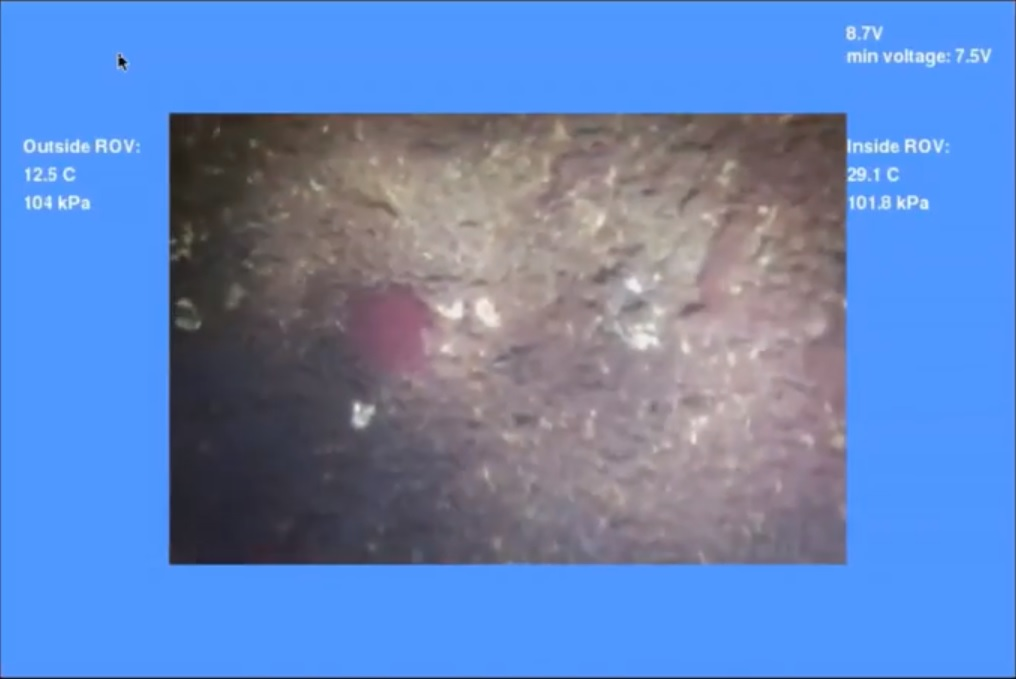
\includegraphics[width=0.8\textwidth]{edurovOld}
    \caption{User interface for the original eduROV software.}
    \label{edurovOld}
\end{figure}

Five main goals were set for my contribution to the project:

\begin{itemize}
\item Reduce the video latency as much as possible while still having the possibility for high resolution images.

\item Streamline the installation process, i.e. remove the need for visiting any website or manually coping files.

\item Remove the need for any third party applications, that would mean removing the RealVNC dependency for video transfer.

\item Increase customization while still maintaining a high level application programming interface (API).

\item Make the UI more attractive, include more UI features without overwhelming the operator.
\end{itemize}

\section{Current alternatives}

There exists a wealth of software's created for operating ROV's. This discussion will be limited to those that are open source and created in Python. The most well known and probably most used is the \emph{Robot Operating System} (ROS)\footnote{\url{http://www.ros.org/}} which is ported to Python as a client library called \emph{rospy}\footnote{\url{http://wiki.ros.org/rospy}}. Although a powerful framework, it does not not suit the needs of this project. Originally written C++, ROS was originally not created for Python. This means that the documentation is mostly in C++ and for anyone who wanted to customize the eduROV software in the future would have learn ROS in addition to Python. It was decided that making ROS fit the needs of the eduROV project would require more time and be limiting to the development, in comparison to creating a tailored software from scratch.

There is also a software called \emph{GoPiGo}\footnote{\url{https://www.dexterindustries.com/gopigo3/}}. This started as a Kickstarter project and is now a hardware and software project that you can buy online. It provides robot communication with video feed, but the software seems to be created specifically for the robots they sell and not as a package meant for other users to build on.

In summary, there wasn't really any good software alternatives for the eduROV project. Actually, I was not able to find any Python packages created for ROV communication with video support built in. There are many guides on the internet that will walk you through how to create this, but the whole process can be really intimidating for people with limited experience. In addition, many of the guides online require you to install multiple software's and download files from additional places. Not very user friendly. Also, in the guides online they often control ROV's by pushing buttons on a screen, not by keyboard input. Lastly, they contain limited to none documentation.

\section{Development}

All popular and well known packages in the Python community is developed in correspondence with the \emph{Python Packaging User Guide}\footnote{\url{https://packaging.python.org/}}. This guide establishes multiple rules on how packages should be developed and distributed. In comparison it is always possible to upload code to a remote repository and ask people to download it from there. But there are many good reasons why any serious actors use this method. 

By distributing code through the \emph{Python Package Index}, anyone can install the package by running \texttt{"pip install edurov"} in a terminal. No need to visit any websites or copy any files. This command will download and install the required files automatically. Second reason is that this greatly simplifies the process of documentation. By creating special files as stated by the guidelines, a separate website with all the documentation is created and uploaded automatically. It also specifies rules for a versioning scheme. This let's the developer create alpha, beta, release candidates and deployment versions of the software. It makes it easy to make sure that everything is tested properly before it get's publicly available.

Git version control was used throughout the project. All the code was uploaded to the remote repository at \url{https://github.com/trolllabs/eduROV}. Git branches was used for rapid prototyping of different ideas. This meant that different approaches were developed concurrently in each their branch. They were then removed one after another as it became clear that the approach did not meet the requirements. The finished package code can also be seen in the appendix, \hyperref[appCode]{section B} on page \pageref{appCode}.

In the first phase of the development two main methods were tested. The first method was based upon the \emph{pygame} package. It required the operator to install Python and the eduROV package on both the ROV and the controlling computer itself. When the software was started a program window would pop up on the controlling computer and display the video feed. Any customization to the features and UI would require the user to learn pygame since all the graphics are created using the pygame API. The original software also used pygame, but this approach did not rely on RealVNC for transmission. Instead it used socket communication to transfer data.

The second method was based upon a web server approach. This method served a web page from the ROV which could then be viewed on any device connected to the same network as the ROV. This meant that the operator would not have to install any software on his or hers computer. It also meant that the UI would be created using html and css instead of pure pygame. This approach were chosen for the new eduROV package. It would completely remove the need to install anything on the operators computer. It would make it possible to view the video stream at multiple devices at the same time. In addition, web browsers has been around for a very long time and much effort has been spent on making them as efficient and flexible as possible. By using the browser as a medium it's possible to take advantage of this. Some high schools also have web development and html as part of their curriculum. By basing the the eduROV package on a web server framework it becomes possible to let the operator customize the UI with their knowledge of html and css.

When the main method were chosen, proceeding development were administered through the \emph{GitHub issues workflow}\footnote{\url{https://github.com/trolllabs/eduROV/issues}}. \figref{issues} shows a section of the \emph{issues} page on GitHub. On this page, feature requests and bug descriptions were posted by me and one other that tested the software. These were then completed in turn and uploaded as \textit{commits} and \textit{releases}.

\begin{figure}[h!]
    \centering
    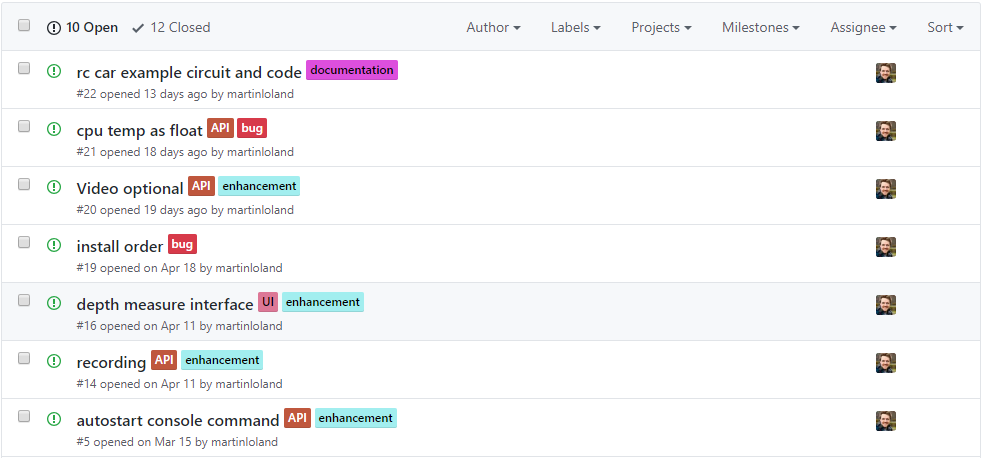
\includegraphics[width=0.8\textwidth]{issues}
    \caption{GitHub eduROV issues overview.}
    \label{issues}
\end{figure}

\section{Architecture}

The eduROV package is based upon a HTTP web server framework. This means that any information sent between the ROV and the user is communicated though HTTP GET requests. For increased performance and robustness many of the different tasks are spread on multiple processes running in parallel. This ensures utilization of multiple CPU cores. The Pyro4\footnote{\url{https://pythonhosted.org/Pyro4/}} Python package uses socket TCP communication and were chosen to facilitate transfer of data between processes. It's fast, well maintained and easy to use.

\figref{edurovArchitecture} pictures the flow of information between different processes and parts of the system. When the user interact with the keyboard, this is sent as a HTTP request from the web browser to the web server on the ROV. This is a threaded HTTP server, which means that multiple requests can be handled at the same time in different computer threads. The web server will forward this information to the \textit{synchronize process} which is responsible for holding an updated version of all variables. The \textit{Arduino process} checks the synchronize process many times per second and forwards any new key presses to the Arduino through a serial connection, which then moves the motors correspondingly. Sensor values moves in a similar fashion, only in the opposite direction. The camera captures frames, compresses them to .jpg files and store them in a memory buffer. The webserver will then send the image to the web browser as soon it is ready, directly from the buffer. Lastly, the \textit{system monitor process} regularly checks that the drive space and CPU temperature is ok and notifies the synchronize process.


\begin{figure}[h!]
    \centering
    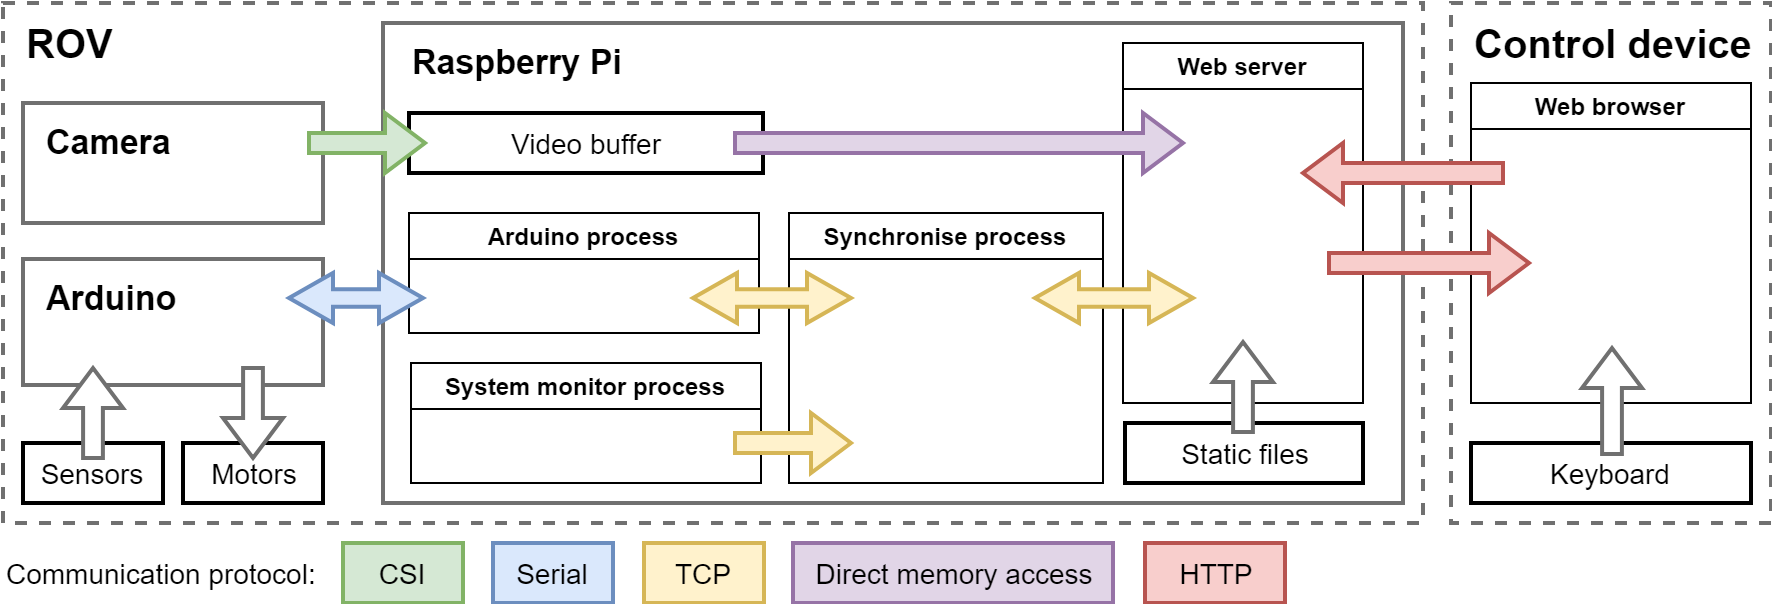
\includegraphics[width=\textwidth]{edurovArchitecture}
    \caption{System architecture of the eduROV software.}
    \label{edurovArchitecture}
\end{figure}

\section{Graphical user interface}

\figref{edurov_gui} shows the finished UI. The layout is dynamic which means that it will fit any screen size and ratio. The side panels will stay the same size, but the video will shrink and increase in size to what's available. Left panels shows sensor values from the Arduino and RPi. Center section shows the video feed. There is also a roll indicator that shows how the ROV is oriented in the water. This indicator can be toggled on/off from the button menu in the right panel. From this panel the operator has multiple options, such as to arm the robot. If the robot is not armed it will not move. Cinema mode will hide all panels and scale the video feed to its maximum size. Some of the actions can also be triggered with hotkeys. With this layout, the user can chose whether to view all information or nothing except the video feed. An approach with information in side panels was chosen because \citet{Chen2007} argued that "overlaying information on video feed can potentially lead to cognitive tunnelling".

\begin{figure}[h!]
    \centering
    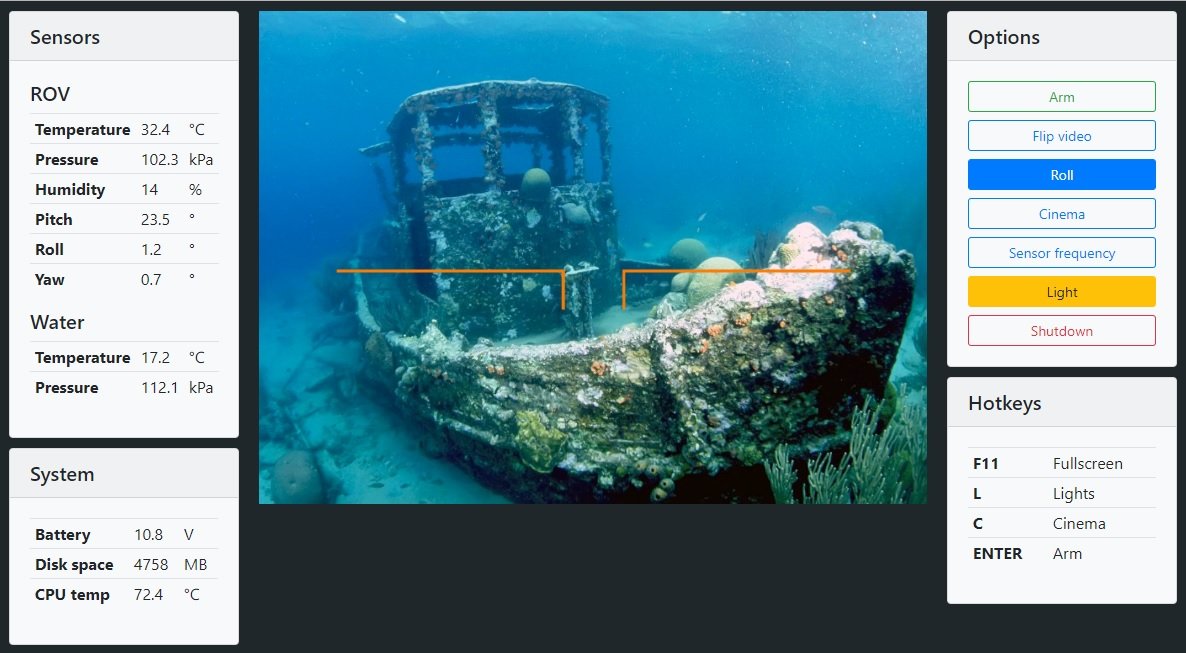
\includegraphics[width=0.8\textwidth]{edurov_gui}
    \caption{The graphical user interface in the eduROV package.}
    \label{edurov_gui}
\end{figure}

The UI seen above is in the context of the Engage eduROV submersible. But since the UI is created purely in HTML, CSS and JavaScript, any user of the package can customize the look and feel of the webpage in any way he or she would like. In fact, a completely different UI was created for the experiment in chapter \ref{chpMethod}, but still used the eduROV framework for handling requests.

\section{Application programming interface}

The application programming interface (API) is how the user interact with the software package. One of the goals of the project was to create an API that would get the user up an running in a matter of minutes. In addition, provide a flexible API that provides extensive flexibility and customization. There is one single main class called \texttt{WebMethod}. By initiating this class with the path to the \texttt{index.html} file which decribes the layout, the web server will start running and serving the web page and video feed. In addition to that, the user is able to customize which functions that should be started in their own processes, custom responses to GET methods, resolution and frame rate and much more.

The reader is recommended to take a look at the API\footnote{\url{http://edurov.readthedocs.io/en/latest/api.html}} and getting started\footnote{\url{http://edurov.readthedocs.io/en/latest/started.html}} section of the documentation. These pages describes the API and provide a much better user experience than what can be provided in a book. 


\section{Documentation}


The documentation is written using the \emph{reStructuredText}\footnote{\url{http://docutils.sourceforge.net/rst.html}} markup syntax and compiled using the Sphinx\footnote{\url{http://www.sphinx-doc.org/}}. This enables in-line program documentation. This is very helpful because the documentation for the classes, methods and functions can be written in the same place as the actual code. This creates fewer files which are easier to maintain. In addition, sphinx will automatically detect classes, functions and methods and create a corresponding documentation structure.

The GitHub repository has been connected to an account at \emph{readthedocs.io}. By connecting these accounts, a documentation website is automatically created from the sphinx structure when updates are committed to the repository. The documentation can be seen online\footnote{\url{http://edurov.readthedocs.io}} or in the appendix, \hyperref[appDoc]{section A} on page \pageref{appDoc}. A sample can be seen in \figref{docs}.

\begin{figure}[h!]
    \centering
    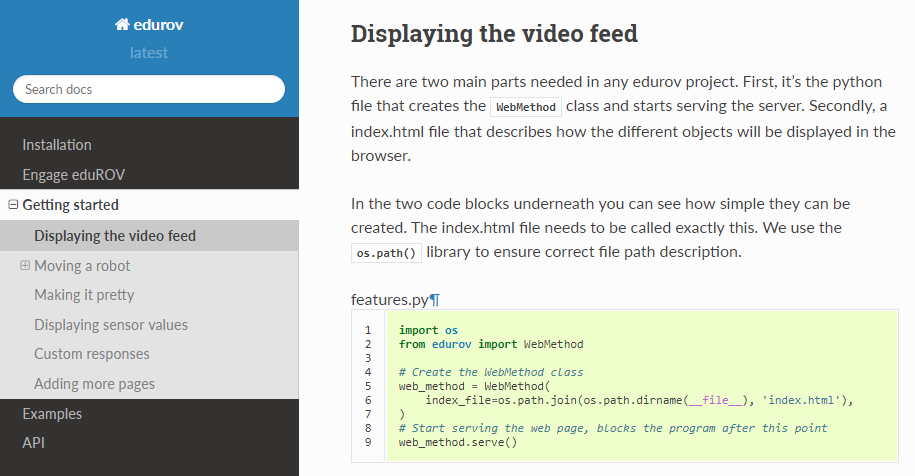
\includegraphics[width=0.8\textwidth]{docs}
    \caption{eduROV documentation at readthedocs.io}
    \label{docs}
\end{figure}
\clearpage
\section{Performance and novelty features}

\begin{figure}[h!]
    \centering
    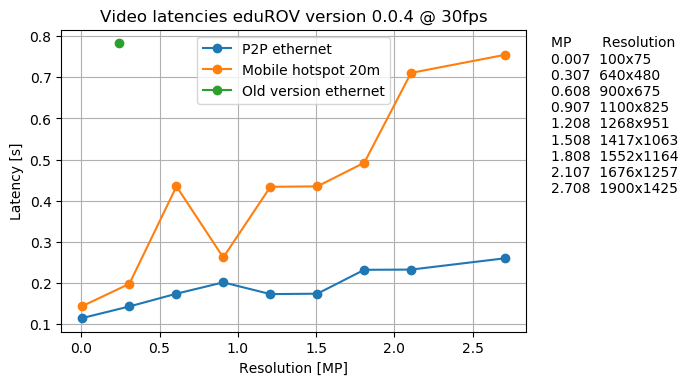
\includegraphics[scale=0.7,right]{latency}
    \caption{Video latency for eduROV 0.0.5 \@ 30fps.}
    \label{latency}
\end{figure}

\figref{latency} shows a delay performance test that were performed on version 0.0.5 of the eduROV package. With a resolution of 0.3 mega pixels on a wired ethernet connection, the video latency has been reduced from 782ms to 143ms. This is a 82\% reduction. It is even possible to stream full HD video with a latency below 300ms. When using wireless transmission the latency is affected by factors such as distance, interference and hardware. The test was performed in the same way as \citet{Jennhag2016} did in their test. By manually comparing two timers, one in real time on the monitor and the other as captured by the camera and transmitted back to the same monitor.
\clearpage
A summary of the most novelty features in comparison with other similar solutions can be listed as follows:

\begin{description}
\item[Low video latency.] Possibility to stream high definition video with a delay below 200ms.

\item[No setup required.] The controlling computer does not need any software installed. The ROV can even be controlled from a mobile phone.

\item[Very easy to use.] One command in the terminal window will install all required files. One additional command will start the web server.

\item[Highly customizable.] Since the UI is created in html the user can customize the look and feel of the web page in any way.

\item[Easy true parallelism.] Custom functions can be spawned on multiple CPU cores while still maintaining the possibility to share variables.
\end{description}

For future work there is one limitation to the current design. The client browser communicates with the web server with GET requests. Each time the UI is updated, the client has to ask for this update, there is no way that the server can send new information to the client on its own. This is unless a \emph{WebSocket} connection is used. Instead of creating a new connection each time a request is done, a websocket is open as long as the client is viewing the web page. This enables the server to push information when it have something new and thus removing a lot of unnecessary communication. This would probably require comprehensive changes to the underlying workings of the eduROV package, but is probably where the next big performance gain can be achieved.	
	
\chapter{Predictive Display Scheme}\label{chpPredictive}
	This chapter describes the developed predictive display. The final results only requires a few lines of code and can be applied to most ROVs. In the coming explanation a very simple and limited ROV is considered, but section \ref{expand} describes how the principle can be expanded to more complicated configurations.

\section{Robot configuration} \label{chp31}
 
To explain how the predictive display (PD) works, let us consider the self balancing two wheeled robot depicted in \figref{twoWheeled}. The upper part of the figure shows the robot from above with two objects in front of it, a black cube and a gray barrel. The ROV is drawn at time equal to $t=0$ and $t=\Delta t$. The bottom part of the image depicts the viewport of the onboard camera mounted to the ROV.


\begin{figure}[h!]    
    \centering           
    \def\svgwidth{.75\columnwidth}
    \input{img/twoWheeled.pdf_tex}
    \caption{Two wheeled robot before and after counter clockwise rotation.}
    \label{twoWheeled}
\end{figure}


It has a forward facing camera with a FOV of $\phi$ degrees. The camera captures a video feed with a resolution of $R_h$ pixels horizontally. Its center of rotation is located in the vector $z$ pointing out of the paper. It is able to rotate with an angular velocity of $\omega$ deg/sec around its center of rotation $z$.

Let us first consider a situation without delay and where the ROV can only be given two commands, to turn either left or right. The commands are given by pressing one of two buttons, not by a joystick with variable output. If the operator holds down the \emph{left} button for a period of $\Delta t$ seconds, the ROV would make an angular rotation of $\omega \cdot \Delta t = \Delta \theta$ degrees. This is depicted in the right side of \figref{twoWheeled}.

In the viewport, the cube and barrel would move to the right as the ROV turned left. These objects has moved a finite number of pixels horizontally $\Delta P_h$, which can be calculated by Equation \ref{deltaph}. It is simply the ratio between the angular rotation and the FOV, times the pixel screen width. By substituting in the expression for angular rotation, Equation \ref{pixelturnrate} is obtained. Here $\eta$ is used to denote the \textit{pixel turn rate}; the pixel rate at which objects in the video moves left or right when the operator turns the ROV.

\vspace{7mm}
\begin{equation}\label{deltaph}
\Delta P_h = \frac{\Delta \theta}{\phi}\cdot R_h
\end{equation}
\vspace{7mm}
\begin{equation}\label{pixelturnrate}
\Delta P_h = \left ( R_h\frac{\omega }{\phi} \right )\Delta t = \eta \cdot  \Delta t
\end{equation}
\vspace{0mm}

$\eta$ is a constant and depending on the screen resolution, camera FOV and the angular velocity of the ROV. By multiplying this factor by the amount of time the operator holds down the left or right button, the number of pixels the objects in the frame should move is obtained.

\section{Predictive visualization}

Let us now consider a situation where there is a $t_d$ seconds delay from when the commands are given by the operator, to the changes can be seen in the video feed. This is the \emph{total perceived delay} described in the introduction, section \ref{timeDelay}. For simplicity, let us also consider a situation where $\Delta t < t_d$.

\figref{movie} shows a representation of what the video feed would look like as the above maneuver was performed. It shows the situation in three different scenarios. First no delay, secondly with delay and third with the PD implemented using the delayed video. The outer rectangle shows the limitations of the monitor, while the inner rectangle is the video feed itself.

\begin{figure}[h!]    
    \centering           
    \def\svgwidth{.8\columnwidth}
    \input{img/movie.pdf_tex}
    \caption{Operator view. Outer box total screen size, inner box video feed.}
    \label{movie}
\end{figure}

\figref{timePlot} plots the visible angular rotation $\alpha$ for the no delay display and the delayed display as a function of time. For the no delay display, visible angular rotation is equal to ROV angular rotation $\alpha = \theta$. In addition, the horizontal image pixel displacement $P_h$ is plotted with the same time axis.

The PD works by moving the video feed on the operator screen the opposite way of what the ROV is moving. The amount of pixels the video $P_h$ is moved is calculated by Equation \ref{pixelturnrate}. In addition, the video is moved back (the same way as the ROV is moving) after $t_d$ seconds has passed. This makes the objects in the video feed appear in the correct position on the operator screen as if there were no delay. Note that the black box in \figref{movie} predictor display center column is in the correct position relative to the no delay display. This approach does however assume that the commands will be properly followed by the ROV. But since the prediction is merely an alteration to the last image received, the prediction errors are not cumulative.


\begin{figure}[h!]    
    \centering           
    \def\svgwidth{\columnwidth}
    \input{img/timePlot.pdf_tex}
    \caption{Visible angular rotation and horizontal image pixel displacement as a function of time.}
    \label{timePlot}
\end{figure}

\vspace{-3mm}
\section{Implementation}

Algorithm \ref{predictorAlg} shows the pseudocode for how this PD is implemented in practice. The horizontal pixel displacement $P_h$ is initialized as zero. Then, the \textsc{predictor display} function is called at a set interval $dt$. The rate of these calls should happen at least as fast as the frame rate of the video (fps). With a fps of 30, the interval should be $dt <= 1/30 \approx 33 ms$. The change in horizontal pixel displacement $\Delta P_h$ is then calculated from Equation \ref{pixelturnrate} and the interface is updated with the new $P_h$. In addition, an asynchronous call is done on the \textsc{move back} function so that the video is moved back to its original position after $t_d$ seconds has passed. It has to be an asynchronous call so that the main program is not blocked when the \textsc{move back} function is waiting.

\newgeometry{bmargin=0mm}
\begin{algorithm}
\caption{Predictive display}\label{predictorAlg}
\begin{algorithmic}[0]
\State $P_h$ = 0 \Comment{horizontal pixel displacement}
\State \Call{set interval}{predictor display, $d t$} \Comment{calls function at interval}
\State

\Function{predictor display}{}
\If{left}
	\State $\Delta P_h$ = $-\eta \cdot d t$ \Comment{equation \ref{pixelturnrate}}
\ElsIf{right}
	\State $\Delta P_h$ = $+\eta \cdot d t$ \Comment{equation \ref{pixelturnrate}}
\Else
	\State $\Delta P_h$ = 0
\EndIf

\State $P_h$ += $\Delta P_h$
\State \Call{update interface}{$P_h$}
\State \Call{move back}{$\Delta P_h$} \Comment{asynchronous call}

\EndFunction
\State

\Function{move back}{$\Delta P_h$}
\State wait $t_d$
\State $P_h$ -= $\Delta P_h$
\EndFunction

\end{algorithmic}
\end{algorithm}


\figref{predictorvis} shows the predictor display as it was implemented in the experiment, which is explained in chapter \ref{chpMethod}. It contains the video feed from the ROV, in addition to a red arrow to visualize the prediction. The operator has recently turned the ROV to the right, and as a result the video has moved to the left. The red arrow has not moved and works as an indication of where the ROV will be heading when the video feed has caught up with the time delay.

\begin{figure}[h!]
    \centering
    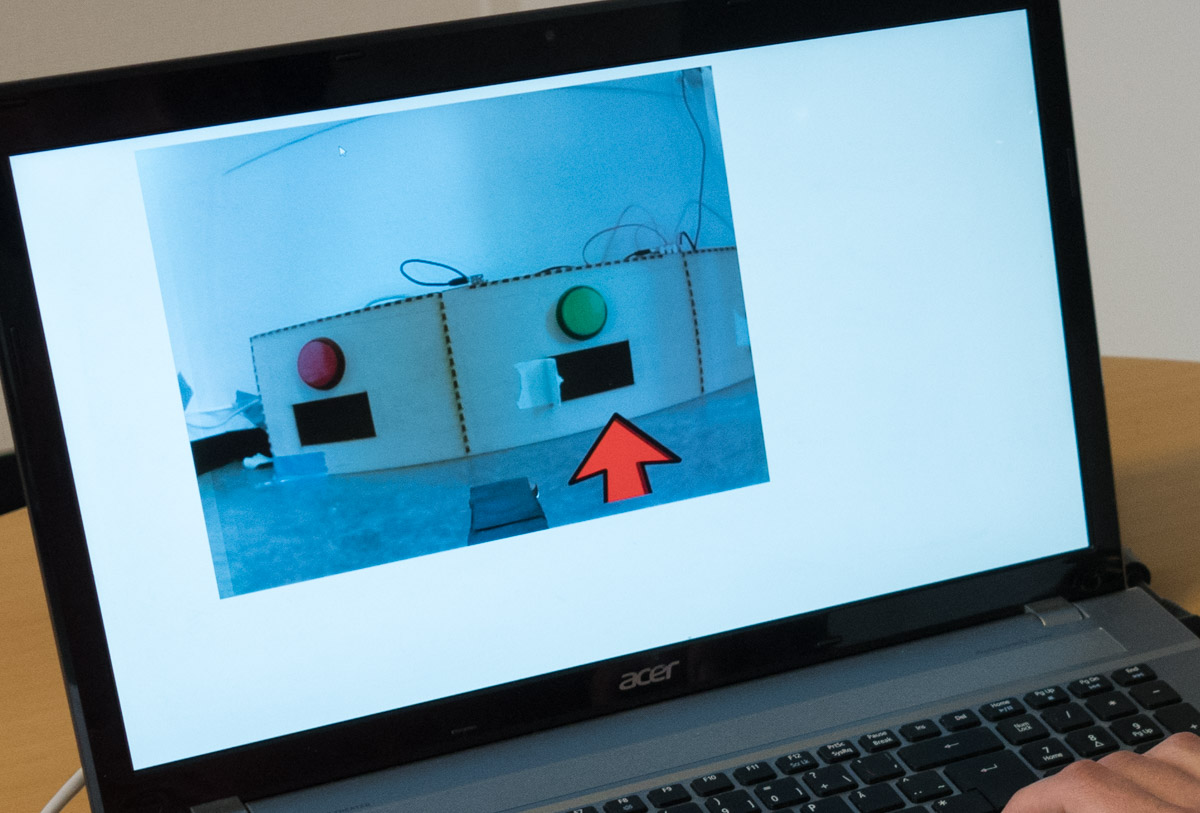
\includegraphics[width=0.7\textwidth]{setup-4}
    \caption{Predictor display visualization.}
    \label{predictorvis}
\end{figure}

\clearpage
\restoregeometry

The operator views the predictor screen through a web browser. The predictor algorithm is written in java script and the video feed is moved around by changing css margin properties. The code can viewed in its entirety in \hyperref[appPredict]{Appendix C} on page \pageref{appPredict}, or online.\footnote{\url{https://github.com/trolllabs/eduROV/blob/master/examples/experiment/displays/predictive.js}}


\section{Extending and generalizing}\label{expand}

The pixel turn rate $\eta$ described in section \ref{chp31} was related to the rotation of the ROV. A similar constant can be found for the \emph{pixel scale rate}, which relates how the the video should be scaled when the ROV moves back and fourth. It's a bit more complicated since the apparent scaling of objects in the frame depends on how far away they are, but by using an average distance this can at least be approximated. The same approach as in Algorithm \ref{predictorAlg} can then be used for backward and forward motion to manipulate the scale of the video feed.

In the case of a varying magnitude of left, right, forward and backward movements, such if the operator is using a joystick with variable output, the PD has to account for this. This can be achieved by applying an adjustment factor to the pixel turn/scale rate proportionate to the magnitude of the command.

The predictor display can then be applied to all moving ROVs. It is just a matter of finding the correct pixel turn/scale rate and adjustment factors corresponding to how the ROV is moving. A submersible ROV would typically have a much lower pixel turn/scale rate because of water friction.

These rates and factors can be found by calculation using ROVs physics and screen resolution. But they can also be found using trial and error. For example, if the visual angular rotation is less than the actual angular rotation, increase the pixel turn rate until they match. In this way, the predictor display can be calibrated without knowing any of the ROVs physics. In this context, \emph{ROV physics} means how the ROV respond to operator input, how fast it moves and turns.	

\chapter{Experiment}\label{chpMethod}
	The goal of the experiment was to measure the performance change in a maneuvering task using a predictor display based on image transformation on a real ROV. The participants were given a modified "peg-in-hole" task, where the peg was mounted on a remotely controlled ground vehicle and the holes were rectangular holes in a wooden box.

%A camera was mounted on the ROV such that the operator could see the peg and holes. The goal of the experiment was to measure the operator's navigational performance difference using two different display types. Both displays would use the same fixed delay, but the second would use predictive technology to visualize instant robot responses. The first display would contain a delayed video feed from an ROV while the other display used predictive visualization with the same delay. The participants were given a task of maneuvering the UGV to three specific locations as many times as possible in the course of 90 seconds.

\section{Participants}

The participants were voluntary selected from the NTNU Department of Mechanical and Industrial Engineering. A total of 58 participants performed the experiment whereas the first one were excluded from the data foundation. This was due to lack of information that became evident during the first trial. This information were given to the other 57 participants. None of the participants had any earlier experience with predictive displays.

35.1\% of the participants were female and the total group had an average age of 24.7 years with an standard deviation of 1.45. 100\% of the group reported that they use a computer on a daily basis. When asked how often he or she play video games (computer or console), the distribution were as follows: daily 4\%, weekly 26\%, monthly 14\%, yearly 30\% and never 26\%.

\section{Experimental design}

\subsection{Equipment}

\begin{figure}[h!]
    \centering
    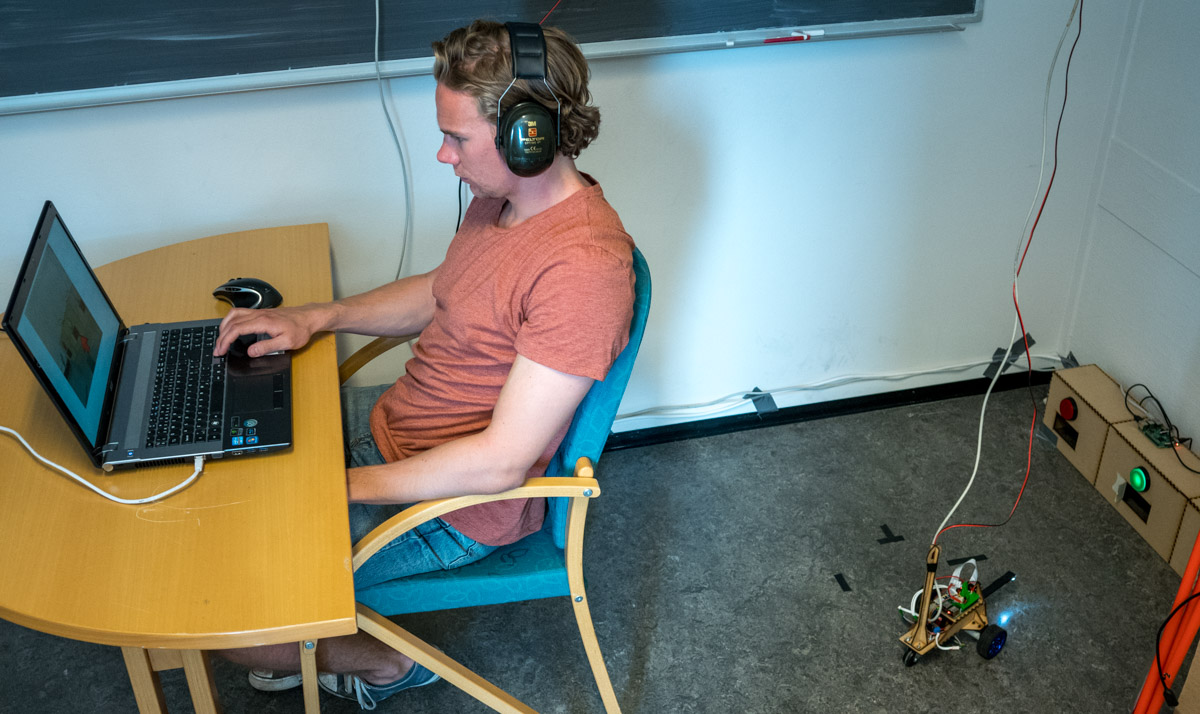
\includegraphics[width=0.8\textwidth]{setup-2}
    \caption{Experimental setup.}
    \label{expsetup}
\end{figure}

\figref{expsetup} shows an overview of the experimental setup. A 17 inch laptop running with a 2.3GHz Intel Core i7-3610QM CPU and Windows 10 together with the arrow keys were used as the operator's control device. This was connected to the ROV through a direct Ethernet connection. 

The ROV, \figref{setup3}, was a three wheeled robot running a Raspberry Pi 3 Model B+. Two of the wheels where connected to each their DC-motor while the third one was a caster wheel for support. The ROV was equipped with a forward facing Raspberry Pi Camera V2. The camera ha a wide angle lens attached with a horizontal FOV of $76.5$ degrees. The robot was running the eduROV software outlined in chapter \ref{chpEdurov}. This software was responsible for serving the control interface, handling control commands, logging experiment data and adding the desired latency to the communication.

A wooden box with three holes and LED's were used to register task performance. The distance between the holes (center to center) was $D=30cm$ while the holes itself has a width of $W=10cm$. This translates to a Fitts's \emph{index of difficulty} of $I_d=log_2\left ( 2D/W \right )=2.58\: bits$ \citep{Fitts1954}.

\subsection{Task}\label{task}

One by one, i random order, the round LED on the button box would turn on. The operator was then tasked to maneuver the ROV such that the black peg would go inside the corresponding hole. A light sensor inside the hole would register this as a \emph{hit}. This would cause the LED to turn off and one of the other two to turn on. The participants were told to make as many \emph{hits} as possible in the course of 90 seconds.

The participants would repeat this task a total of three times, using three different displays / conditions. The order of these conditions followed a 3x3 Latin Square Design, to eliminate the order effect. Condition one had a total delay of 700 ms which included the inherent delay of the system 250ms, plus the added delay of 450 ms. Condition two had the same delay as condition one, but with the predictive display in effect. The third condition had no added delay and only the inherent delay of 250ms. No predictive technology was used in the third condition. The total latency of 700 ms were chosen because it's below the reported threshold for a "move and wait" strategy \citep{Chen2007} and above what is considered a difficult level in many situations.

\begin{figure}[h!]
    \centering
    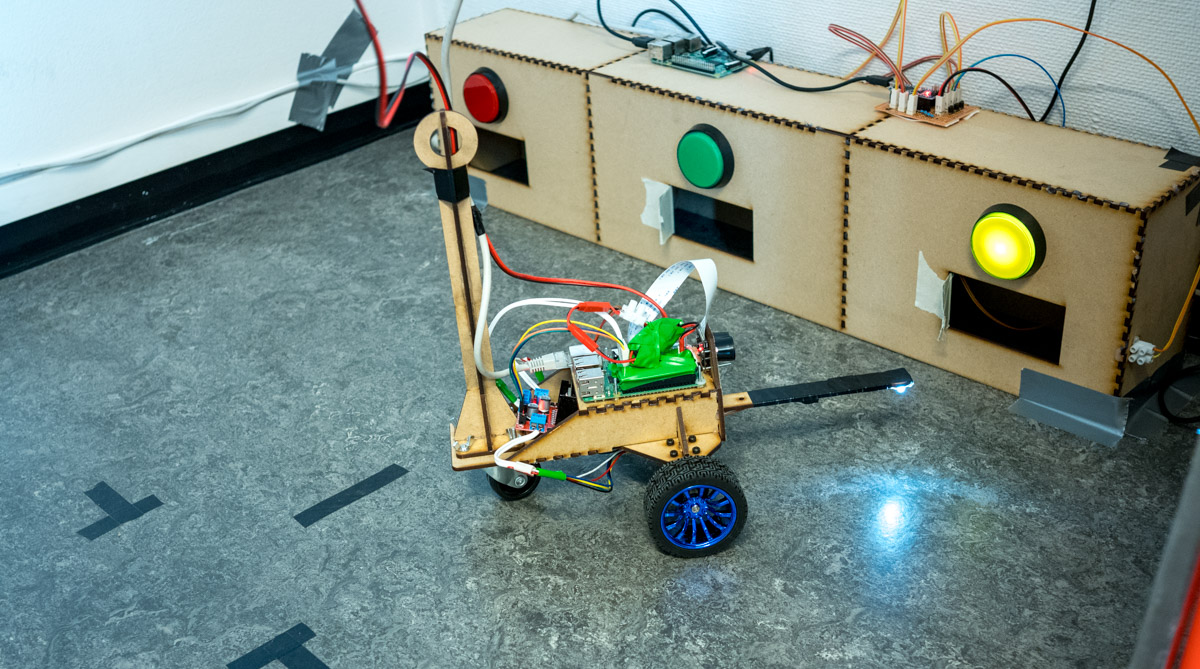
\includegraphics[width=0.65\textwidth]{setup-3}
    \caption{Three wheeled robot used in experiment.}
    \label{setup3}
\end{figure}

Many of the experiments previously mentioned in table \ref{reviewPred} used a single task and measured the task completion time in different conditions. This experiment however was designed with a single simple task and measured the achieved score in the course of a fixed time period. There are multiple reasons for this choice. 

First, to reduce the learning effect that would accompany a longer maneuvering course. Some of the authors in table \ref{reviewPred} reported that the participants performed better for each try when they started to learn the obstacle course. I believe that a longer course would require more time to reduce the learning effect.

Secondly, \citep{Chen2007} reported that the benefit of PD is very task dependent. An easy task was therefore chosen to minimize the effect that task complexity had on the performance results. 

Thirdly, some experiments with real or simulated driving have long stretches with forward motion. The PD provides little help in these situations but still contribute to the task completion time in the same way. A task which required the operator to move from side to side as much as possible was therefore chosen. In addition, by not letting the operator accelerate to maximum ROV velocity, ceiling effects from vehicle limitations were reduced. 

As a fourth argument, a fixed task time made the experiment length much more predictable. Subjects used on average 10 minutes and 56 seconds with a standard deviation of 1 min and 12 s to perform the whole experiment. This again made it easier to recruit new subjects. 

As a last argument, the combination of score achievement and time pressure made the subjects fully devoted to the task at hand. This made them performed as close as possible to their potential.

\section{Procedure}

After entering the experiment room, the participants were able to look at the ROV with the button box to get a sense of situational awareness. From that point on, the subject was facing the other way, looking at the computer screen and with the robot outside their FOV. The participants also wore an ear protection headset to remove audible feedback. All the necessary information was given on the screen.

First, the subject S was presented with an initial form collecting demographic data and an information page describing experiment theme, how to steer the robot, the participant's goal and how the experiment would proceed. This can be found in the appendix, page \textbf{TODO}. The S was then automatically assigned to a group as defined by subsection \ref{task}. The S then perform a 30 seconds long practice period followed by a 90 seconds long real test. This was done repeatedly for all of the three conditions. At the end of each test, the S was asked to fill out a test questionnaire.  After each practice and test run, the ROV was repositioned to it's original position defined by the black markings in \figref{setup3}.

The S was \emph{not} told that one of the conditions would contain a predictor display or how the predictor display worked.

\section{Data recording and analysis}

All the data was recorded with the onboard computer on the ROV using a SQLite database. This included demographics, experiment questionnaire data, hits made by the subjects, number of key presses and more. Time stamp data was also recorded for each hit and the test start and end. A total of 11865 data points were collected during the testing period.

The test questionnaire that was completed for each condition included a NASA TLX (task load index) form \citep{Hart1988}, in addition the S had to guess the total delay that they just experienced. This questionnaire can be found in the appendix at page \textbf{TODO}. One modification were done to the NASA TLX form. During the preliminary experiment evaluation, a helper reported that he found it naturally to evaluate a good performance with a high score. In the original questionnaire a low values translates to a good performance. This metric and the corresponding description was reversed such that a high value would reflect a good performance. After data collection, this value was reversed back such that it can be reported inline with convention.

The number of hit's made by the S in the course of 90 seconds was used to quantify performance. This score was normalized in the same way as \citep{Rachmielowski2010} and \citep{Lovi2014} did in their analysis. First, the S's number of hits in a specific condition was divided by the total number of hit's in all three conditions. It was then multiplied with the average score in that condition for all participants. The same normalization has also been done on the reported subjective delay for each condition.

To determine the statistical difference between conditions a two-sided paired sample t-test was used. In practice, this was calculated using the \texttt{scipy.stats.ttest\_rel} function which is a part of the SciPy python library. In the results section, the t-statistics is reported as \emph{t}, the two-tailed p-value as \emph{p} and the degrees of freedom $n-1$ as \emph{df}.

When comparing scores based on demographic groups, the variables are no longer dependent. In those cases, a two-sided Welch’s t-test is performed instead. This has been computed using the \texttt{scipy.stats.ttest\_ind} function. The statistics is reported in the same fashion as in the dependent case, only difference is that the degrees of freedom is calculated using the Welch–Satterthwaite equation \citep{Allwood2008}.

The effects size, which describes the magnitude of difference between conditions was calculated using the Cohen's d formula. This value is reported as \emph{d} in the results. The formulas used for the t-test and Cohen's d can be found in the appendix at page \textbf{TODO}.

\todo[inline]{
linear regression

\texttt{scipy.stats.linregress}
}	

\chapter{Results and Discussion}\label{chpResults}
	This chapter will present the results and discussion divided into six consecutive themes: general performance, gaming effects, task load index, subjective delay, learning effects and key presses.

\section{Performance}

\figref{performanceNorm} shows the normalized number of hits in 90 seconds (score), for each display type and all N=57 participants. \textit{Delay} refers to the \textit{added} delay, which means that "No delay" translates to the inherent system delay of $250 ms$. The numerical values are reported in Table \ref{score}. The statistical significance and effect size between conditions can be seen in Table \ref{score2}.

\begin{figure}[h!]
    \centering
    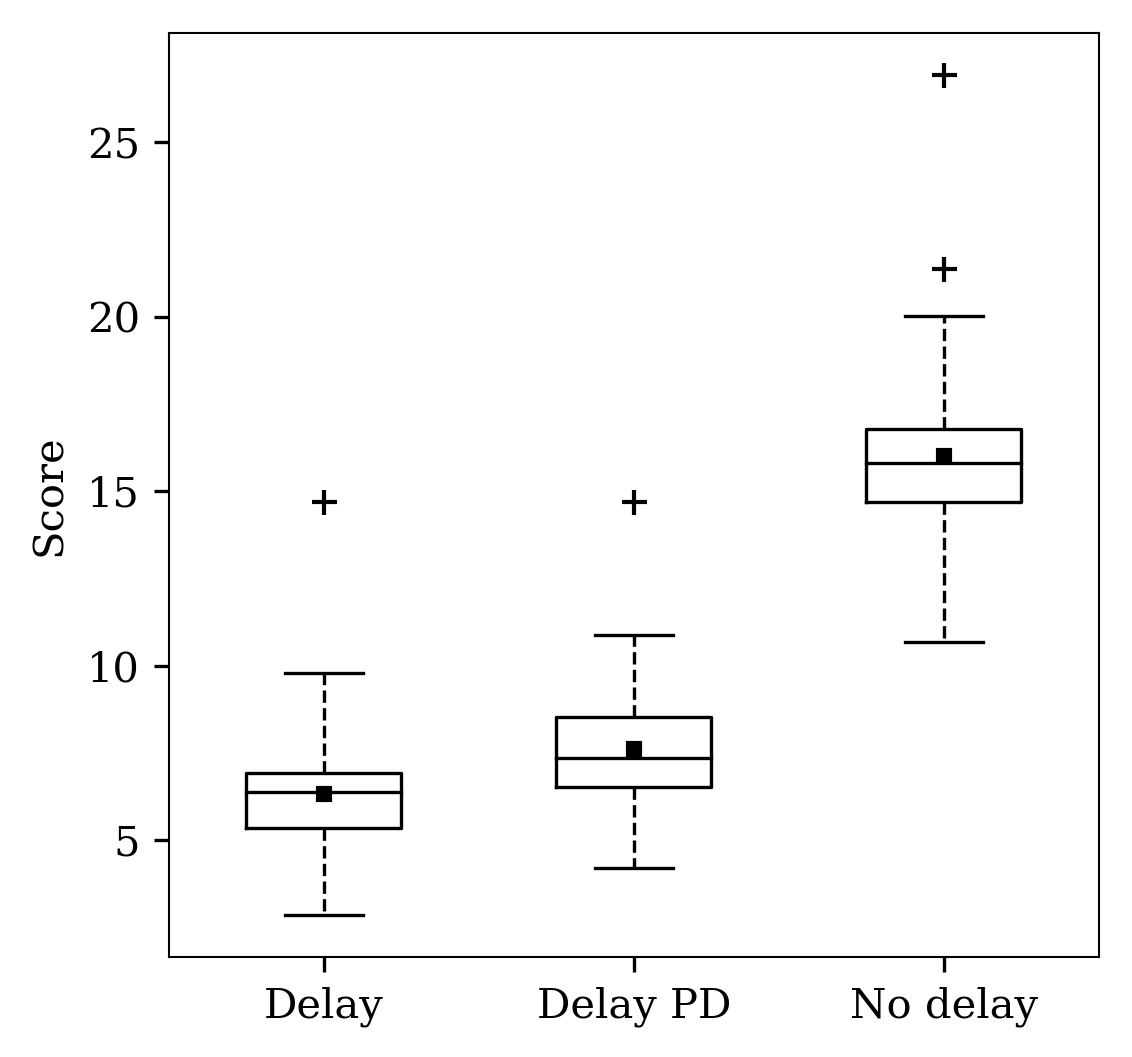
\includegraphics[scale=0.85]{performance_norm}
    \caption{Normalized score all participants, N=57.}
    \label{performanceNorm}
	\vspace{-0.2cm}
\end{figure}

% Please add the following required packages to your document preamble:
% \usepackage{booktabs}
\begin{table}[]
\small
\centering
\caption{Normalized mean scores and standard deviation (SD).}
\label{score}
\begin{tabularx}{\textwidth}{@{}XXXXX@{}}
\toprule
Differentiation & Group       & Display  & Score & SD \\ \midrule
None            & All N=57    & Delay    & 6.24  & 1.39               \\
                &             & Delay PD & 7.52  & 1.43               \\
                &             & No delay & 15.87 & 1.99               \\ \addlinespace
Gender          & Male n=38   & Delay    & 6.65  & 1.25               \\
                &             & Delay PD & 7.95  & 1.43               \\
                &             & No delay & 17.30 & 1.71               \\ \addlinespace
                & Female n=19 & Delay    & 5.39  & 1.49               \\
                &             & Delay PD & 6.61  & 1.35               \\
                &             & No delay & 13.10 & 2.17               \\ \addlinespace
Gaming          & Daily n=2   & Delay    & 7.92  & 0.37               \\
                &             & Delay PD & 10.21 & 1.40               \\
                &             & No delay & 18.36 & 1.77               \\ \addlinespace
                & Weekly n=15 & Delay    & 6.27  & 1.22               \\
                &             & Delay PD & 8.17  & 1.51               \\
                &             & No delay & 17.62 & 2.04               \\ \addlinespace
                & Monthly n=8 & Delay    & 7.05  & 1.32               \\
                &             & Delay PD & 7.77  & 0.64               \\
                &             & No delay & 17.68 & 0.95               \\ \addlinespace
                & Yearly n=17 & Delay    & 6.65  & 1.26               \\
                &             & Delay PD & 7.66  & 1.73               \\
                &             & No delay & 15.98 & 2.25               \\ \addlinespace
                & Never n=15  & Delay    & 5.06  & 1.46               \\
                &             & Delay PD & 6.21  & 1.16               \\
                &             & No delay & 12.73 & 1.79               \\ \bottomrule
\end{tabularx}
\end{table}

% Please add the following required packages to your document preamble:
% \usepackage{booktabs}
\begin{table}[]
\centering
\caption{Paired samples t-test and Cohen's d effect size}
\label{score2}
\begin{tabularx}{\textwidth}{@{}llYYYY@{}}
\toprule
\multicolumn{2}{c}{Pair} & \multicolumn{3}{c}{t-test for Equality of Means} &       \\ \cmidrule(lr){3-5}
\multicolumn{2}{l}{}     & t                  & df             & p                   & d     \\ \midrule
Delay       & Delay PD   & 4.82               & 56             & $<$.001             & 0.735 \\
Delay       & No delay   & 23.04              & 56             & $<$.001             & 4.413 \\
Delay PD    & No delay   & 19.52              & 56             & $<$.001             & 3.861 \\ \bottomrule
\end{tabularx}
\end{table}

\figref{performanceNorm} together with the statistical data in Table \ref{score2} shows that there is a statistical difference in performance when controlling the ROV without and with predictive help. Subjects performed on average 20.6\% better with an effect size of $d=0.904$. This can be categorized as a medium to large effect, especially when considering how easy and cheap this predictive method is to implement.

Past research, Table \ref{reviewPred}, describes a wide range performance gains from predictive technology. Everything from 8\% to 65\%. It's hard to do a direct comparison to any specific experiment, but a performance increase of 20.6\% in this experiment is probably in the lower range of what has been found before. What is true though, is that the predictive method described in this thesis is the cheapest and easiest to implement, at least when comparing to those in Table \ref{reviewPred}.

None of the subjects were told that there would be a predictive display or how it worked. Some of the participants immediately identified what the predictive display was trying to tell them. Others however, didn't understand that there had been a predictive display until the experiment was over. The ones who tried to use the predictive display the way it was intended typically performed better than those who didn't. It may be possible that we could have seen an improved performance, if the subjects were informed how the predictive display works. This can however not be verified unless additional experiments are performed.

\section{Gaming}

Those who play games weekly or more were defined as \emph{gamers} (G). They performed on average 30.13\% better, while non-gamers (NG) only saw a 16.91\% performance increase using the PD. This difference is illustrated in \figref{gamer_performance} and Table \ref{score2}.

\begin{figure}[h!]
	\vspace{-2mm}
    \centering
    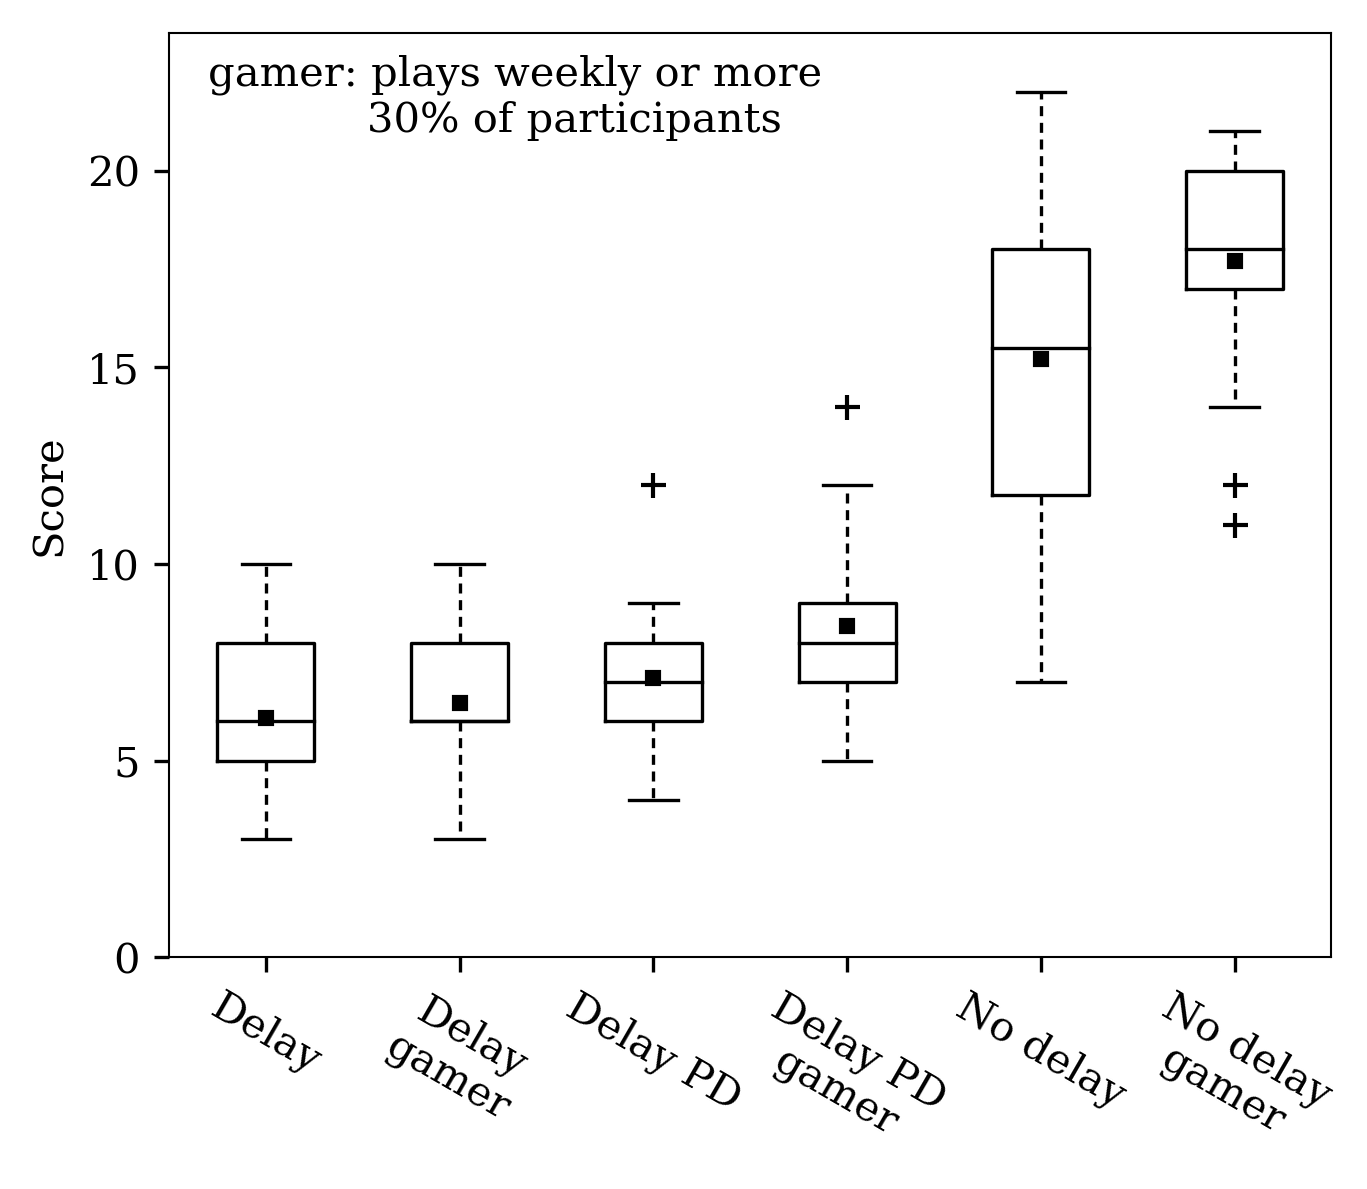
\includegraphics[scale=0.85]{gamer_performance}
    \caption{Performance of gamers n=17, versus non-gamers n=40.}
    \label{gamer_performance}
	\vspace{-3mm}
\end{figure}

It is interesting to see that G's were able to increase their score almost twice as much as NG's when going from a delayed condition to a delayed condition with PD. Exactly why G's were able to increase their performance more using the PD is unclear. It could be that the arrow in the PD which acts like an aiming device, is a more familiar concept for gamers. It could also indicate that G's are generally more adaptable to new an unfamiliar situations in a computer competition setting.

When comparing G's versus NG's directly, it is also interesting to see that G's only performed better than NG's in the second and third condition. Delay PD: t(26.57)=2.23, p=0.034, d=0.692 and no delay: t(40.79)=2.56, p=0.014, d=0.660. In the the first condition, there was no significant difference.

\newgeometry{bmargin=5mm}
\section{Task load index}

\figref{tlx} shows the reported NASA TLX scores. The height of the bar describes the mean value while the whiskers shows the SD. Numerical values are reported in Table \ref{tlx_values}.

Subjects reported minimal differences between condition one and two. The only significant differences were found in performance and frustration. Subjects felt that they on average performed 14\% better using the predictor display, t(56)=3.24, p=0.002, d=0.360. The actual performance increase was 21\%. They also reported that they felt 11\% less frustrated using the PD, t(56)=2.15, p=0.036, d=0.271. Participants also stated that the no delay condition was better in all metrics, with an exception of \emph{temporal demand} where the difference was not significant.

\begin{figure}[h!]
    \centering
    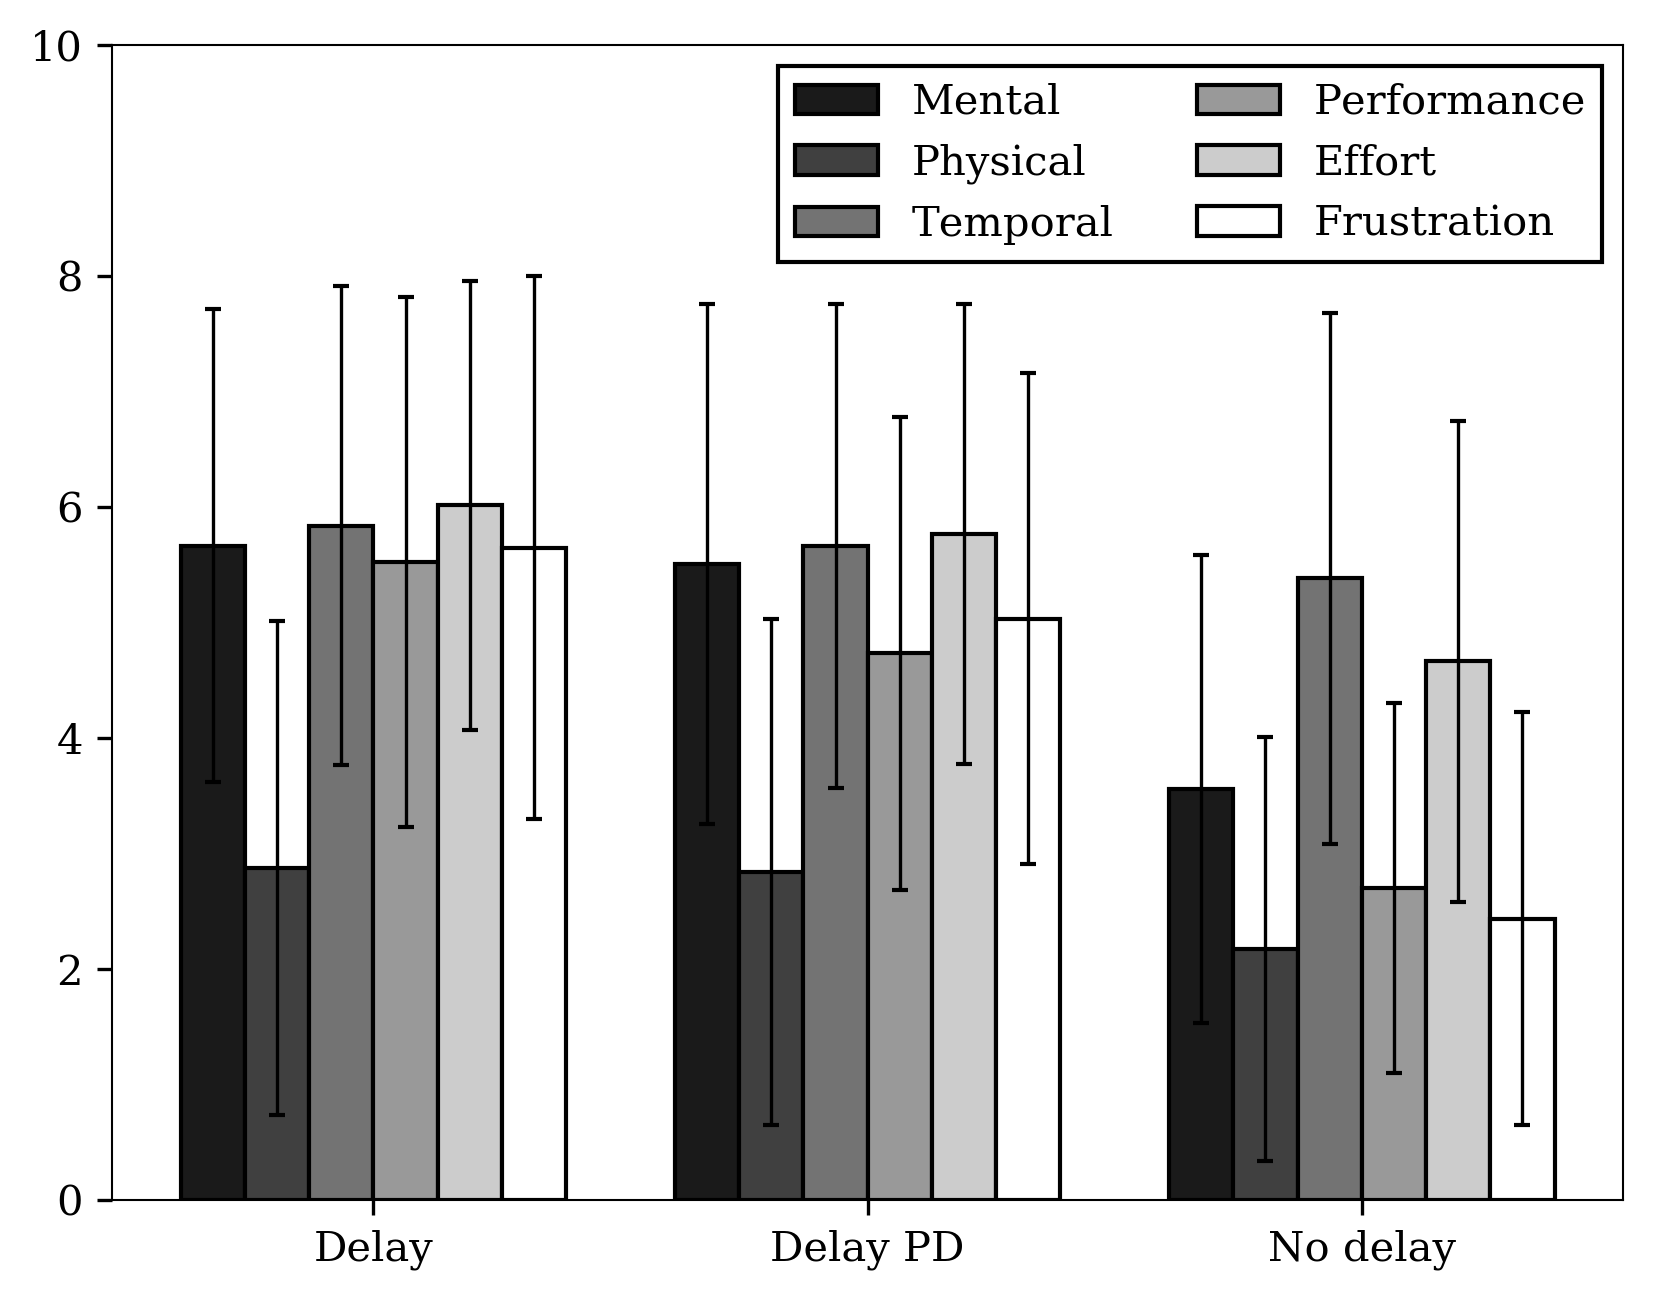
\includegraphics[scale=0.8]{nasa_tlx_bar}
    \vspace{-2mm}
    \caption{NASA TLX (task load index) results for each display type, N=57. Lower is better.}
    \vspace{-3mm}
    \label{tlx}
\end{figure}

The subjects reported no significant difference in mental, physical and temporal demand between condition one and two. These three metrics is a good description of the total subjective workload. Some subjects, especially those who didn't understand what the PD were trying to tell them, even reported the PD as distracting.

\restoregeometry

Because of how the PD works, the video feed is constantly moving around and scaling up and down. This can understandably be distracting. Some participants immediately understood how the PD worked, and they typically reported the PD as helpful. They also seemed to be more relaxed, but there are no recorded data that can prove this relationship.

% Please add the following required packages to your document preamble:
% \usepackage{booktabs}
\begin{table}[]
\small
\centering
\caption{Rated NASA TLX values and standard deviation (SD), N=57. Lower is better.}
\label{tlx_values}
\begin{tabularx}{\textwidth}{@{}llXXllXX@{}}
\toprule
Metric      & Display  & Rating      & SD         &        Metric      & Display  & Rating      & SD                 \\ \midrule
Mental      & Delay    & 5.67        & 2.05       &        Performance & Delay    & 5.53        & 2.29               \\
            & Delay PD & 5.51        & 2.25       &                    & Delay PD & 4.74        & 2.05               \\
            & No delay & 3.56        & 2.03       &                    & No delay & 2.70        & 1.60               \\\addlinespace
Physical    & Delay    & 2.88        & 2.14       &        Effort      & Delay    & 6.02        & 1.94               \\
            & Delay PD & 2.84        & 2.19       &                    & Delay PD & 5.77        & 1.99               \\
            & No delay & 2.18        & 1.84       &                    & No delay & 4.67        & 2.08               \\\addlinespace
Temporal    & Delay    & 5.84        & 2.08       &        Frustration & Delay    & 5.65        & 2.35               \\
            & Delay PD & 5.67        & 2.10       &                    & Delay PD & 5.04        & 2.13               \\
            & No delay & 5.39        & 2.30       &                    & No delay & 2.44        & 1.79               \\ \bottomrule

\end{tabularx}
\end{table}

During the task, a red timer indicating the remaining time was constantly visible for the participant to see in the upper right corner. In addition, the robot had rapid acceleration and was able move fast if the operator managed to do so. Overall, this made for a hectic and exiting experience for the subjects. This may explain why there is no significant change in the temporal demand, even compared to the no delay situation. The fact that the participants reported a better value (smaller) in the other five metrics for the no delay condition, is as expected. This finding supports earlier research that describes how video latency negatively affect the user experience in teleoperation.

\clearpage
\section{Subjective delay}

\figref{subjective_delay_norm} shows the normalized reported total delay in seconds for the three conditions. The participants reported a 11\% decrease in subjective latency using the predictive display versus the normal display with the same latency. This results is however not significant, t(56)=1.40, p=0.167, d=0.356. From the Figure, it can be seen that subjects reported the latency in the third condition as very low, many of them barely above 0ms. The actual delay was 250ms, but only

About 75\% of the participants underestimated the latency in the third condition. Many of them barely reported over 0ms, but the actual latency was 250ms. These findings support previous research, which states that smaller latencies closer to zero is difficult to differentiate from no latency.

\begin{figure}[h!]
    \centering
    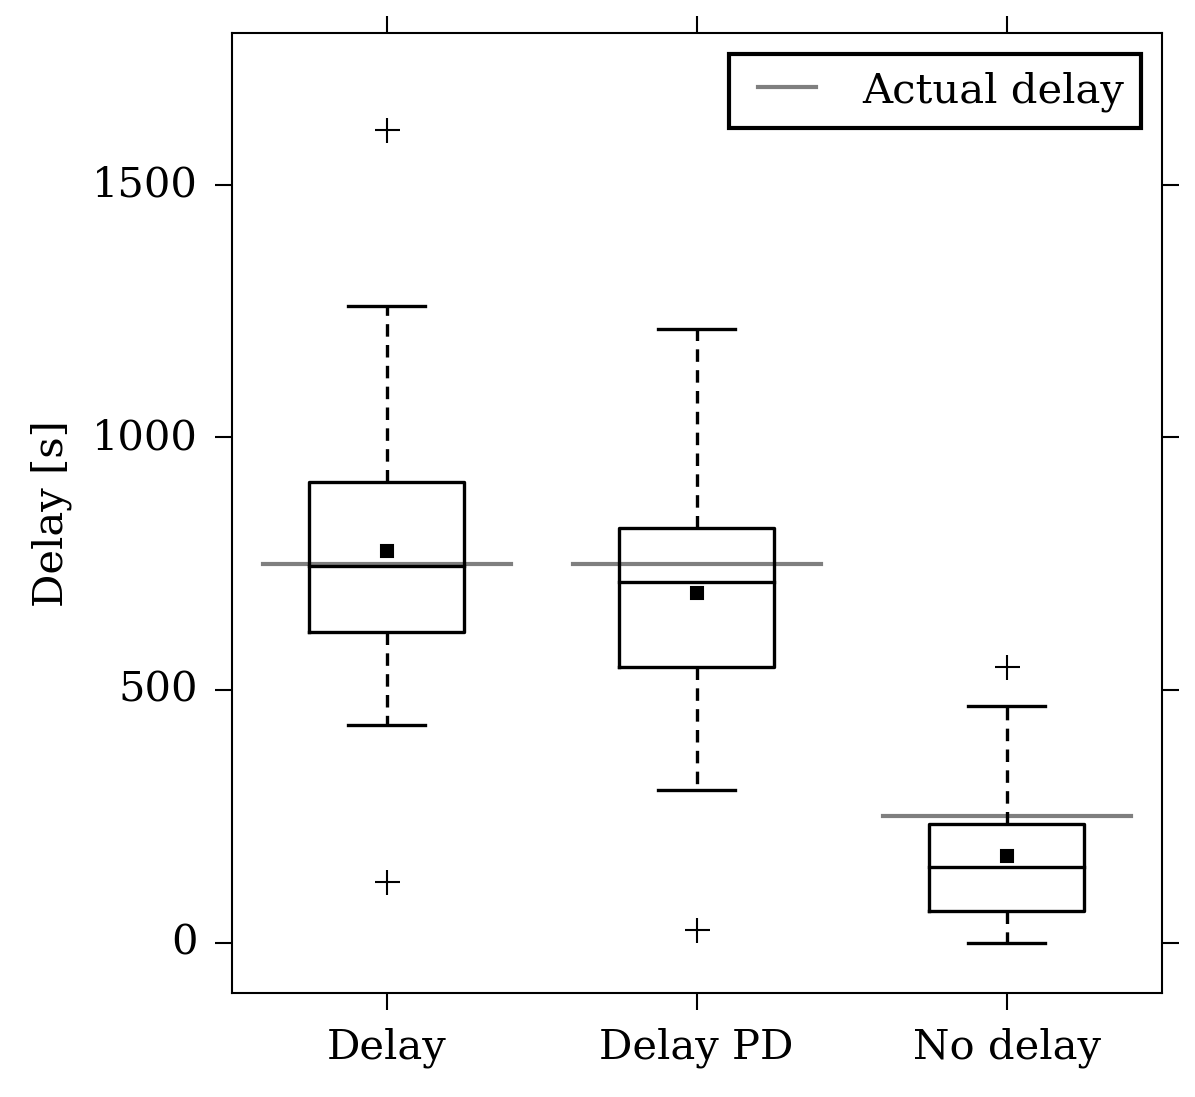
\includegraphics[scale=0.85]{subjective_delay_norm}
    \caption{Normalized reported subjective latency in seconds.}
    \label{subjective_delay_norm}
\end{figure}

\clearpage
Since the participants reported less frustration using the PD, it it interesting to look at how frustration and subjective delay time might be related. \figref{delay_vs_frustration} shows a scatter plot of reported frustration and delay time for all conditions collectively. All values has been normalized. The linear relationship is small, but still noticeable. Note that this Figure presents the subjective latency in all conditions, this means that there are differences between actual latency also. When looking at the different conditions isolated, there are no significant relationships.

\begin{figure}[h!]
    \centering
    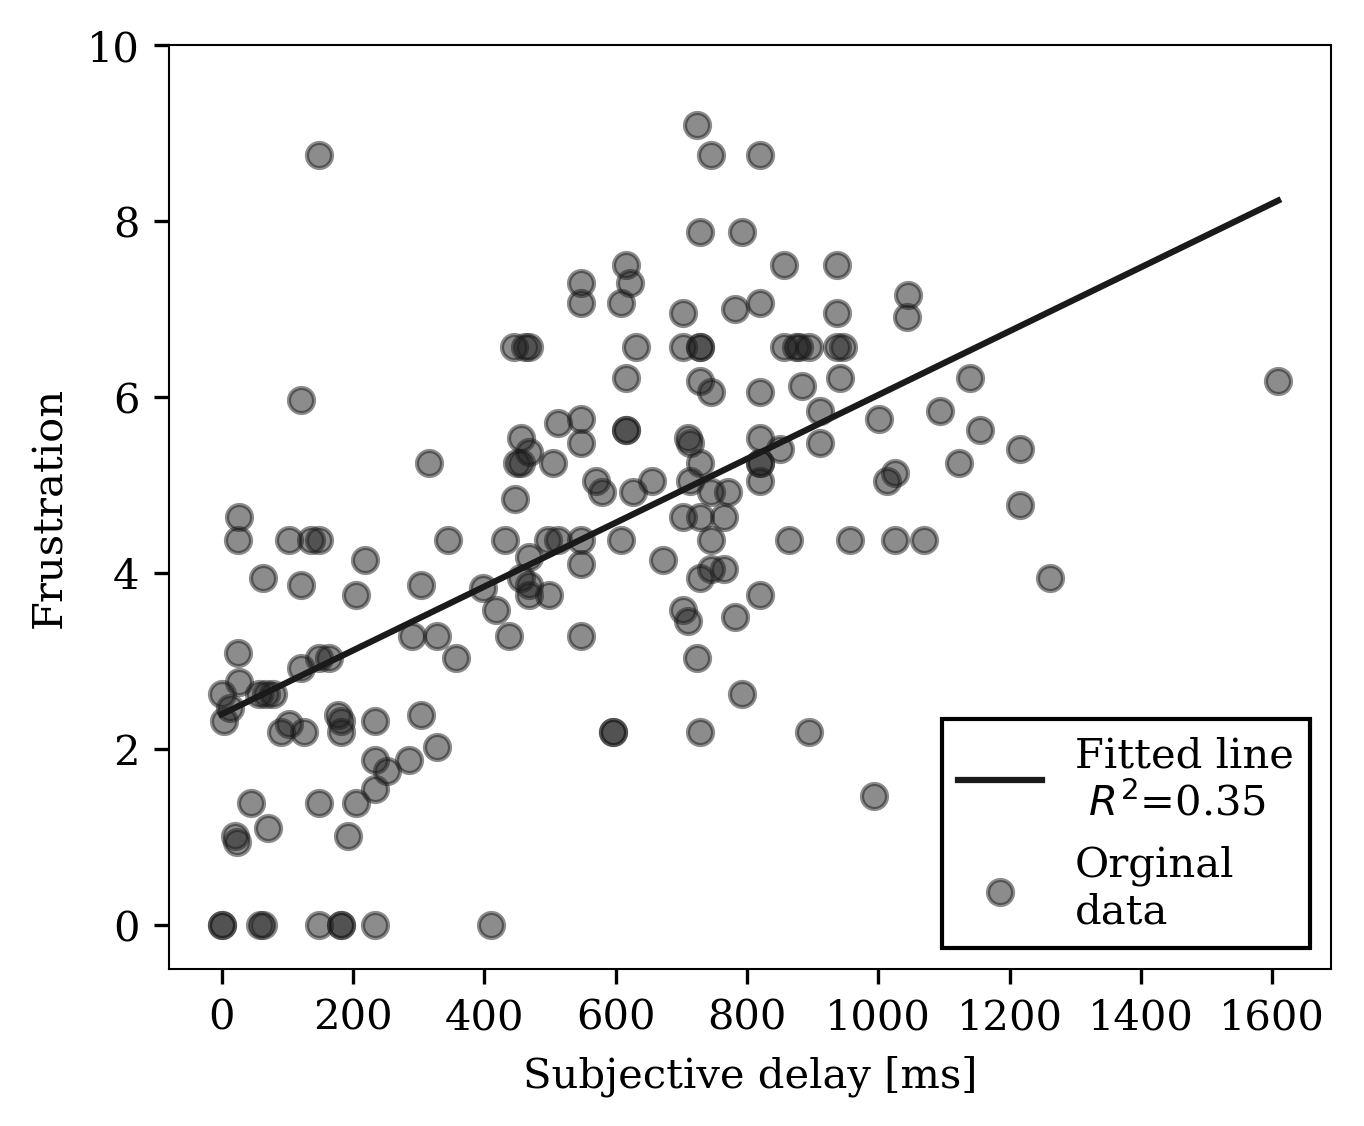
\includegraphics[scale=0.85]{delay_vs_frustration}
    \caption{Normalized subjective delay versus frustration.}
    \label{delay_vs_frustration}
\end{figure}

\clearpage
\section{Learning effect}

It is also interesting the evaluate if participants had any learning effects during the experiment. \figref{learning_effect} shows the score for each display type and further divided into groups depending if the subject had that display as the first, second or third display. As an example, the first of the nine box plots describes the score achieved in the delay condition for those who had that display as their first display. One visible trend is that the participants who had a particular display as their second display, performed better than those who had that display as their first. This performance increase was significant for all displays. Delay: t(18)=2.19, p=0.042, d=0.671, delay PD: t(17)=2.19, p=0.043, d=0.660, no delay: t(17)=3.26, p=0.005, d=0.902. The performance change from \#2 to \#3 in all displays were however not found significant.

This indicate that the participants had some learning effect from the first to second display. But after that, the learning effect was eliminated.

\begin{figure}[h!]
    \centering
    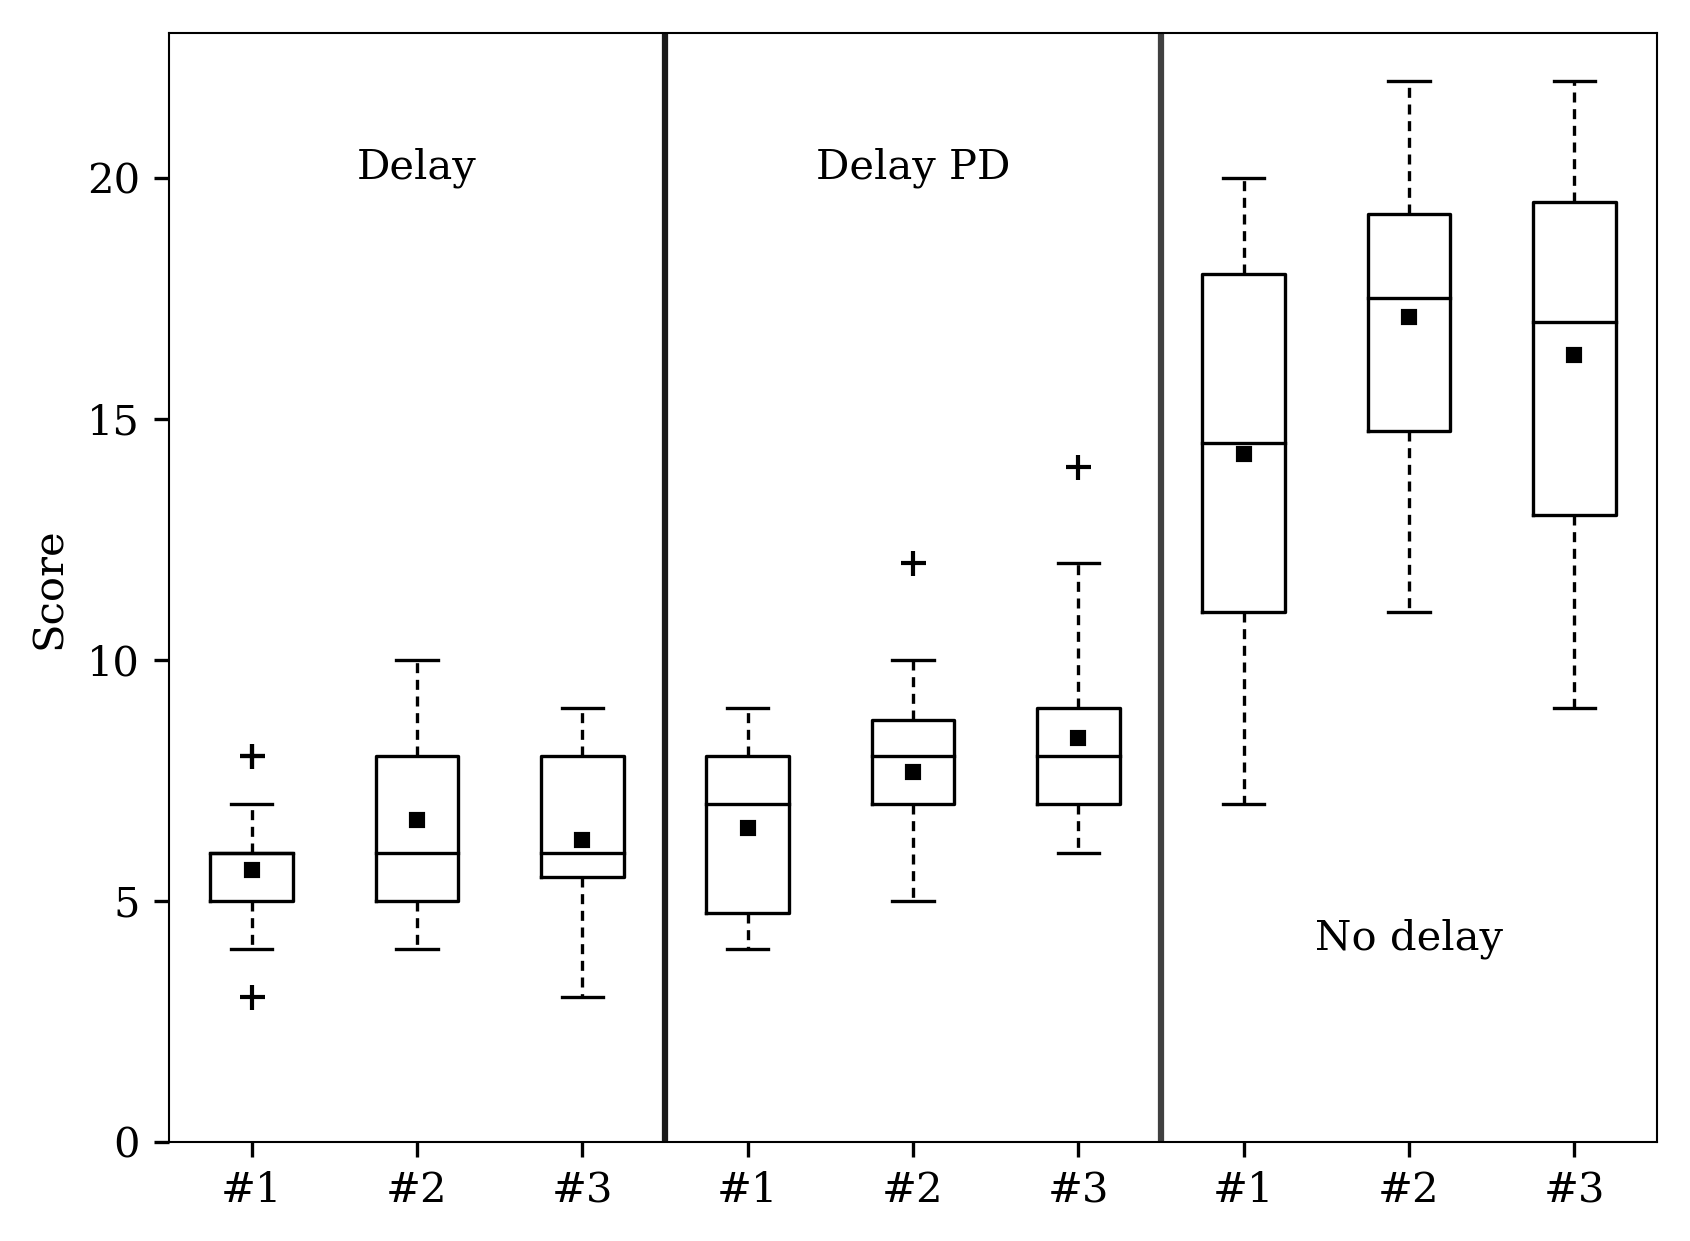
\includegraphics[width=0.85\textwidth]{learning_effect}
    \caption{Score categorized after display order.}
    \label{learning_effect}
\end{figure}

\clearpage
Table \ref{groups_score} and \ref{groups_stats} presents the achieved score in each of the experiments groups. These groups are defined by the 3x3 Latin Square design to minimize order effects. It is interesting to see that the two groups who had condition two, the predictor display first, did not show any statistical difference in performance between condition one and two. But all the other groups who had the PD as their second or third display, showed a performance increase from 24.34\% to 45.58\%. This would indicate that the PD was more helpful, if the subject has tried one of the others first.

\begin{table}[]
\small
\centering
\caption{Mean score and standard deviation (SD) for each group.}
\label{groups_score}
\begin{tabularx}{\textwidth}{@{}XXlXXX@{}}
\toprule
Group   & n  & Display order & Display  & Score & SD   \\ \midrule
Group 1 & 9  & 1-2-3         & Delay    & 5.08  & 1.21 \\
        &    &               & Delay PD & 7.40  & 1.13 \\
        &    &               & No delay & 15.40 & 1.83 \\ \addlinespace
Group 2 & 10 & 1-3-2         & Delay    & 6.24  & 0.72 \\
        &    &               & Delay PD & 8.45  & 0.96 \\
        &    &               & No delay & 17.41 & 1.02 \\ \addlinespace
Group 3 & 10 & 2-1-3         & Delay    & 6.65  & 1.15 \\
        &    &               & Delay PD & 6.32  & 1.03 \\
        &    &               & No delay & 17.04 & 1.51 \\ \addlinespace
Group 4 & 10 & 2-3-1         & Delay    & 6.58  & 1.52 \\
        &    &               & Delay PD & 6.57  & 0.57 \\
        &    &               & No delay & 16.76 & 1.59 \\ \addlinespace
Group 5 & 9  & 3-1-2         & Delay    & 6.78  & 0.91 \\
        &    &               & Delay PD & 8.42  & 1.33 \\
        &    &               & No delay & 14.69 & 1.45 \\ \addlinespace
Group 6 & 9  & 3-2-1         & Delay    & 6.03  & 1.84 \\
        &    &               & Delay PD & 8.04  & 1.45 \\
        &    &               & No delay & 13.59 & 2.58 \\ \bottomrule
\end{tabularx}
\end{table}
% Please add the following required packages to your document preamble:
% \usepackage{booktabs}
\begin{table}[]
\small
\centering
\caption{Mean difference, paired samples t-test and Cohen's d effect size for display pair scores. Seperated by experiment display order.}
\label{groups_stats}
\begin{tabularx}{\textwidth}{@{}lllYYYY@{}}
\toprule
\multicolumn{2}{c}{\begin{tabular}[c]{@{}c@{}}Group / Display order\\ Pair\end{tabular}} & Mean difference & \multicolumn{3}{c}{t-test for Equality of Means} & d      \\ \midrule
\multicolumn{2}{l}{}             &                 & t               & df          & p                &        \\ \cmidrule(lr){4-6}
\multicolumn{2}{l}{Group 1, n=9, 1-2-3}  &                 &                 &             &                  &        \\
Delay           & Delay PD       & 45.58\%         & 4.49            & 8           & 0.002            & 1.867  \\
Delay           & No delay       & 203.00\%        & 10.11           & 8           & $<$.001          & 6.274  \\
Delay PD        & No delay       & 108.13\%        & 8.11            & 8           & $<$.001          & 4.960  \\ \addlinespace
\multicolumn{2}{l}{Group 2, n=10, 1-3-2} &                 &                 &             &                  &        \\
Delay           & Delay PD       & 35.42\%         & 4.89            & 9           & $<$.001          & 2.474  \\
Delay           & No delay       & 179.12\%        & 22.73           & 9           & $<$.001          & 12.050 \\
Delay PD        & No delay       & 106.11\%        & 14.59           & 9           & $<$.001          & 8.602  \\ \addlinespace
\multicolumn{2}{l}{Group 3, n=10, 2-1-3} &                 &                 &             &                  &        \\
Delay           & Delay PD       & -4.98\%         & -0.63           & 9           & 0.544            & -0.288 \\
Delay           & No delay       & 156.29\%        & 12.57           & 9           & $<$.001          & 7.347  \\
Delay PD        & No delay       & 169.73\%        & 13.93           & 9           & $<$.001          & 7.884  \\ \addlinespace
\multicolumn{2}{l}{Group 4, n=10, 2-3-1} &                 &                 &             &                  &        \\
Delay           & Delay PD       & -0.13\%         & -0.01           & 9           & 0.988            & -0.007 \\
Delay           & No delay       & 154.87\%        & 9.99            & 9           & $<$.001          & 6.211  \\
Delay PD        & No delay       & 155.19\%        & 16.53           & 9           & $<$.001          & 8.081  \\ \addlinespace
\multicolumn{2}{l}{Group 5, n=9, 3-1-2}  &                 &                 &             &                  &        \\
Delay           & Delay PD       & 24.34\%         & 2.66            & 8           & 0.029            & 1.366  \\
Delay           & No delay       & 116.81\%        & 11.05           & 8           & $<$.001          & 6.163  \\
Delay PD        & No delay       & 74.38\%         & 6.74            & 8           & $<$.001          & 4.248  \\ \addlinespace
\multicolumn{2}{l}{Group 6, n=9, 3-2-1}  &                 &                 &             &                  &        \\
Delay           & Delay PD       & 33.42\%         & 2.74            & 8           & 0.026            & 1.147  \\
Delay           & No delay       & 125.50\%        & 5.06            & 8           & $<$.001          & 3.190  \\
Delay PD        & No delay       & 69.02           & 4.18            & 8           & 0.003            & 2.503  \\ \bottomrule
\end{tabularx}
\end{table}

\clearpage
\section{Key presses}

\figref{keypresses} shows the number of key presses performed during the 90 seconds of task time for each display type. In condition three participants make a lot more key presses. With a low latency, participants are in a greater degree trying to continuously maneuver the ROV, instead of partially adapting a move and wait strategy.

\begin{figure}[h!]
    \centering
    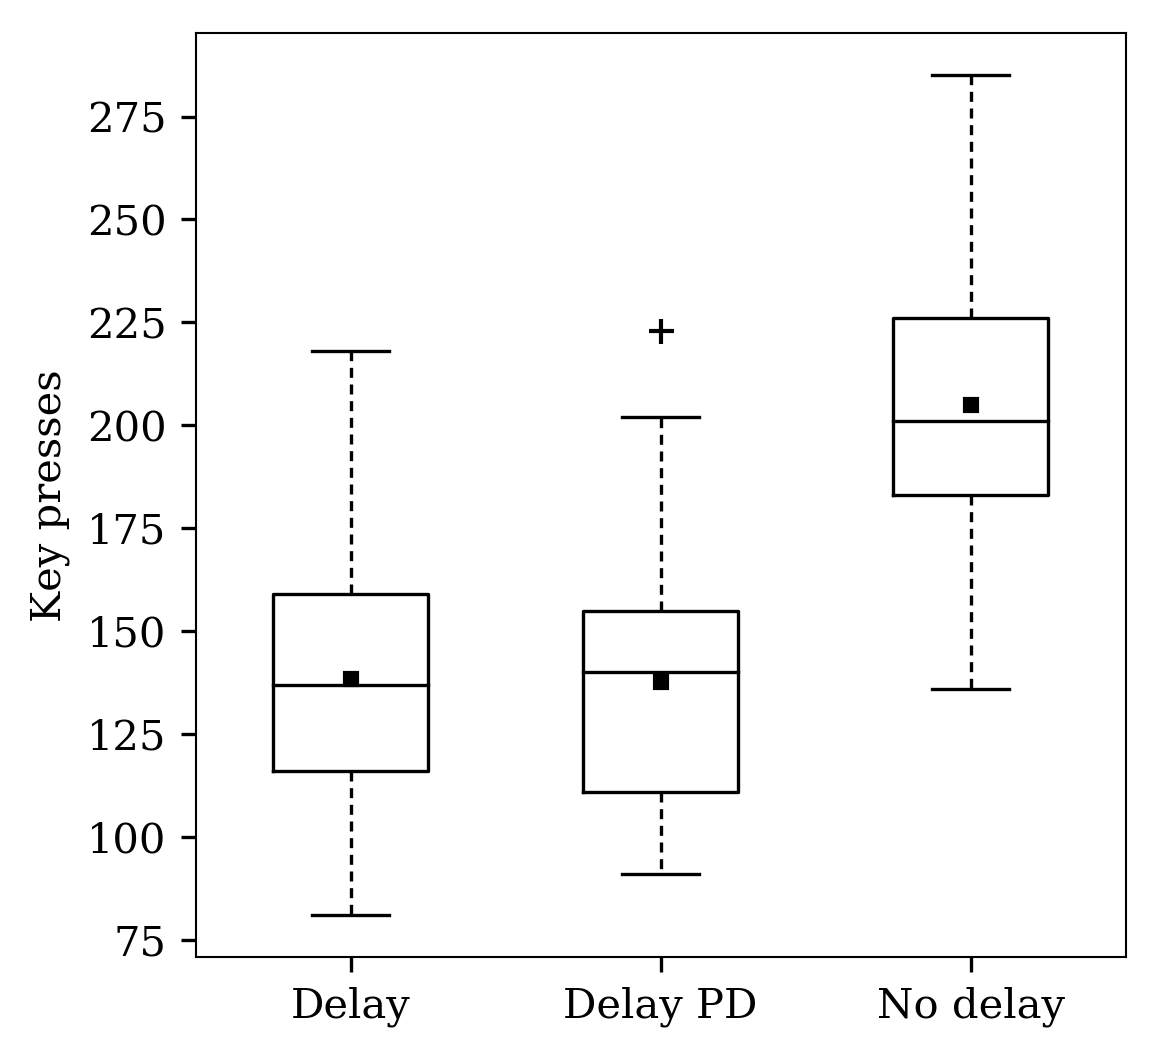
\includegraphics[scale=0.85]{keypresses}
    \caption{The number of key presses performed during 90 seconds.}
    \label{keypresses}
    \vspace{-5mm}
\end{figure}

\section{Limitations}

The choice of not informing the participants about the predictive display before they started the experiment was a conscious one. Because of this, the experiment was limited to testing the performance increase by an \emph{intuitive} understanding of the PD. The results may had been different if the participants were informed in advance. The experiment was also conducted indoors on a flat confined area using a ROV with zero turn radius. More experiments has be performed to evaluate if the results in this thesis are applicable to a real ROV in an unstructured environment.


\chapter{Conclusion and Summary}\label{chpConc}
	\section{Hypothesis}
\todo[inline]{
- Hypothesis

- novelty of solution
}

\section{Future work}
\subsection{Predictive display}
\todo[inline]{
- h264 compression tracking could be used for live improvement of the predictor display

- it might be better to crop with different windows instead of moving the video, people reported that it was disturbing

- many get fixated on the real center pin even though there is a red arrow there, it would be interesting to see if they performed better without any real reference

- wider FOV

- live machine learning to better predict the movement (speed, incline, battery power etc.)
}
\subsection{eduROV package}
\todo[inline]{
- websockets

- flask?
}

{\setstretch{1.0}
}
\printbibliography[title=References]
\addcontentsline{toc}{chapter}{References}

\begin{appendices}\label{appendix}

\chapter*{eduROV documentation}\label{appDoc}
\addcontentsline{toc}{section}{A eduROV Documentation}
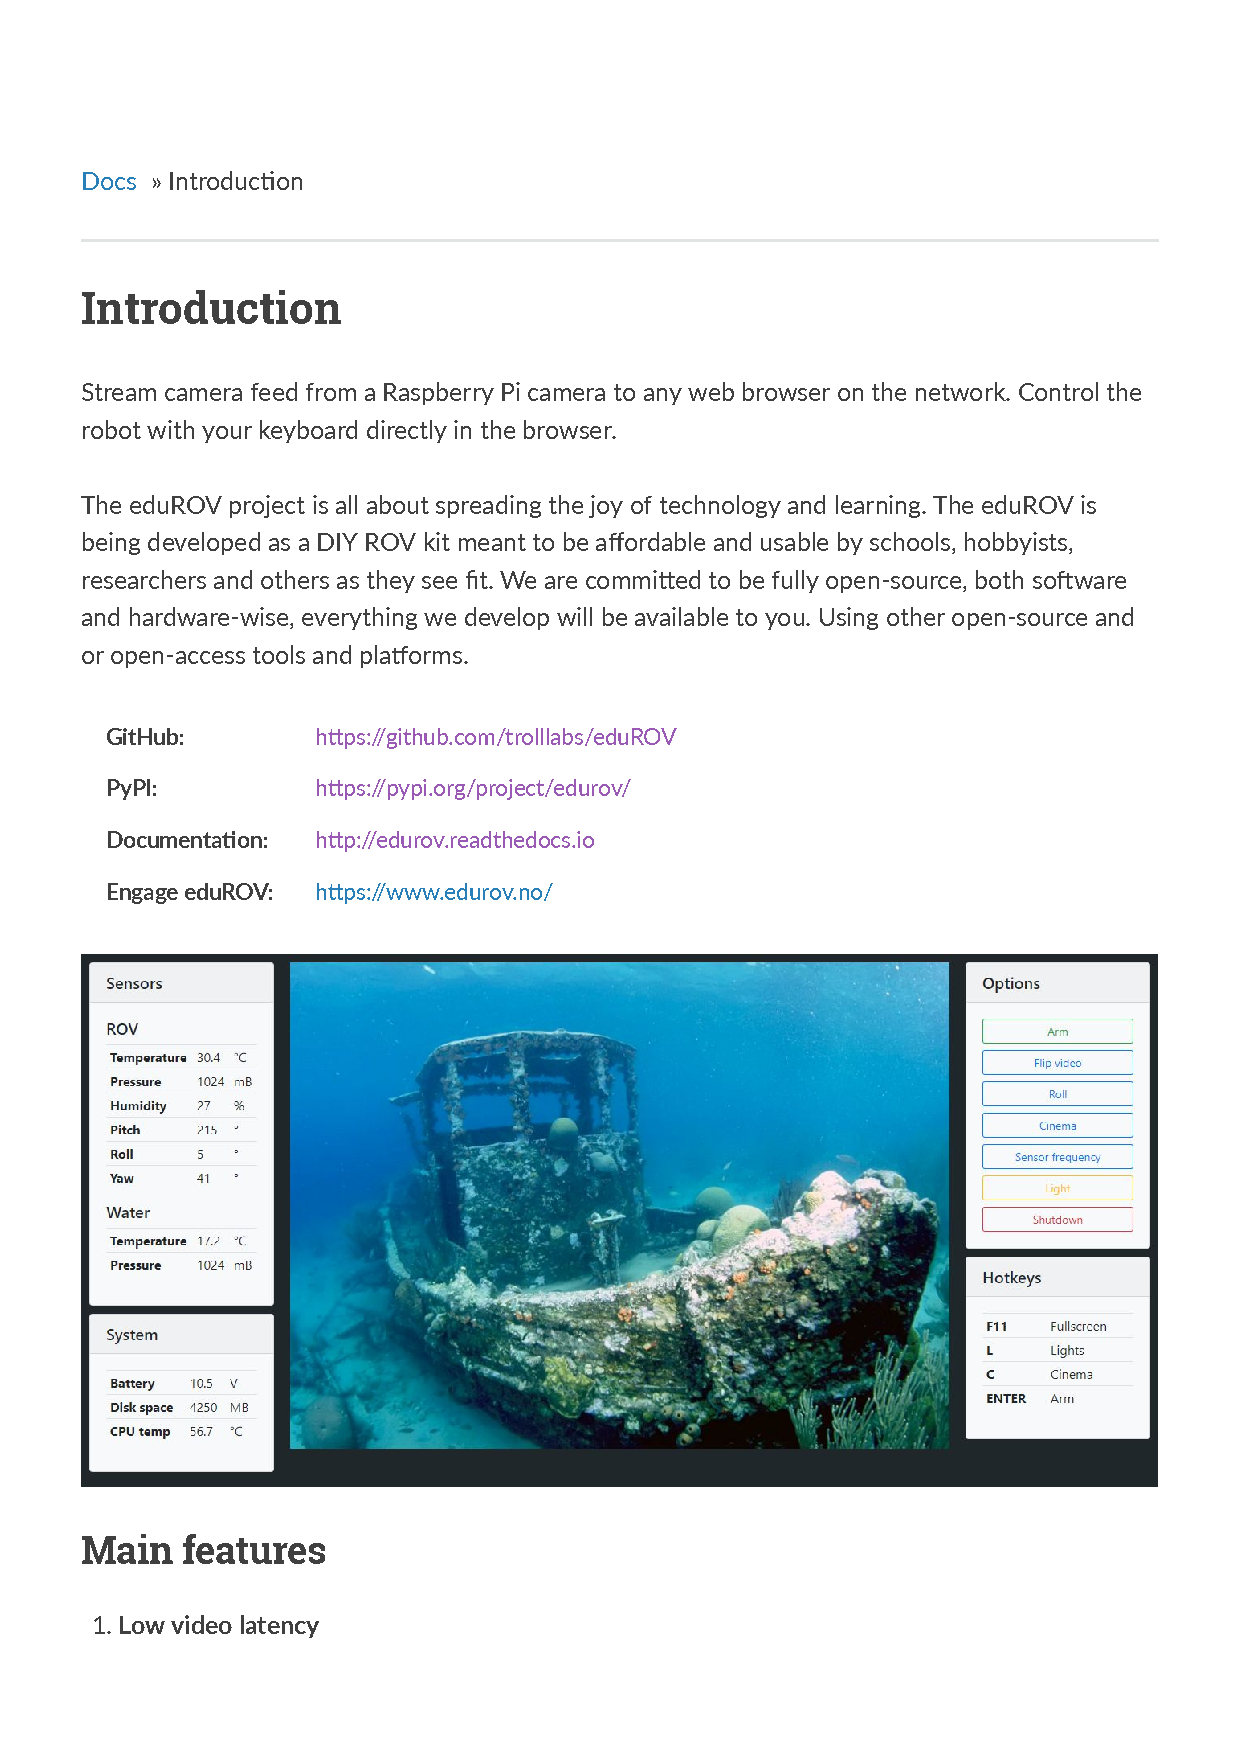
\includepdf[pages=-, frame=false, pagecommand={}, width=0.9\paperwidth]{./appendicies/docP1.pdf}
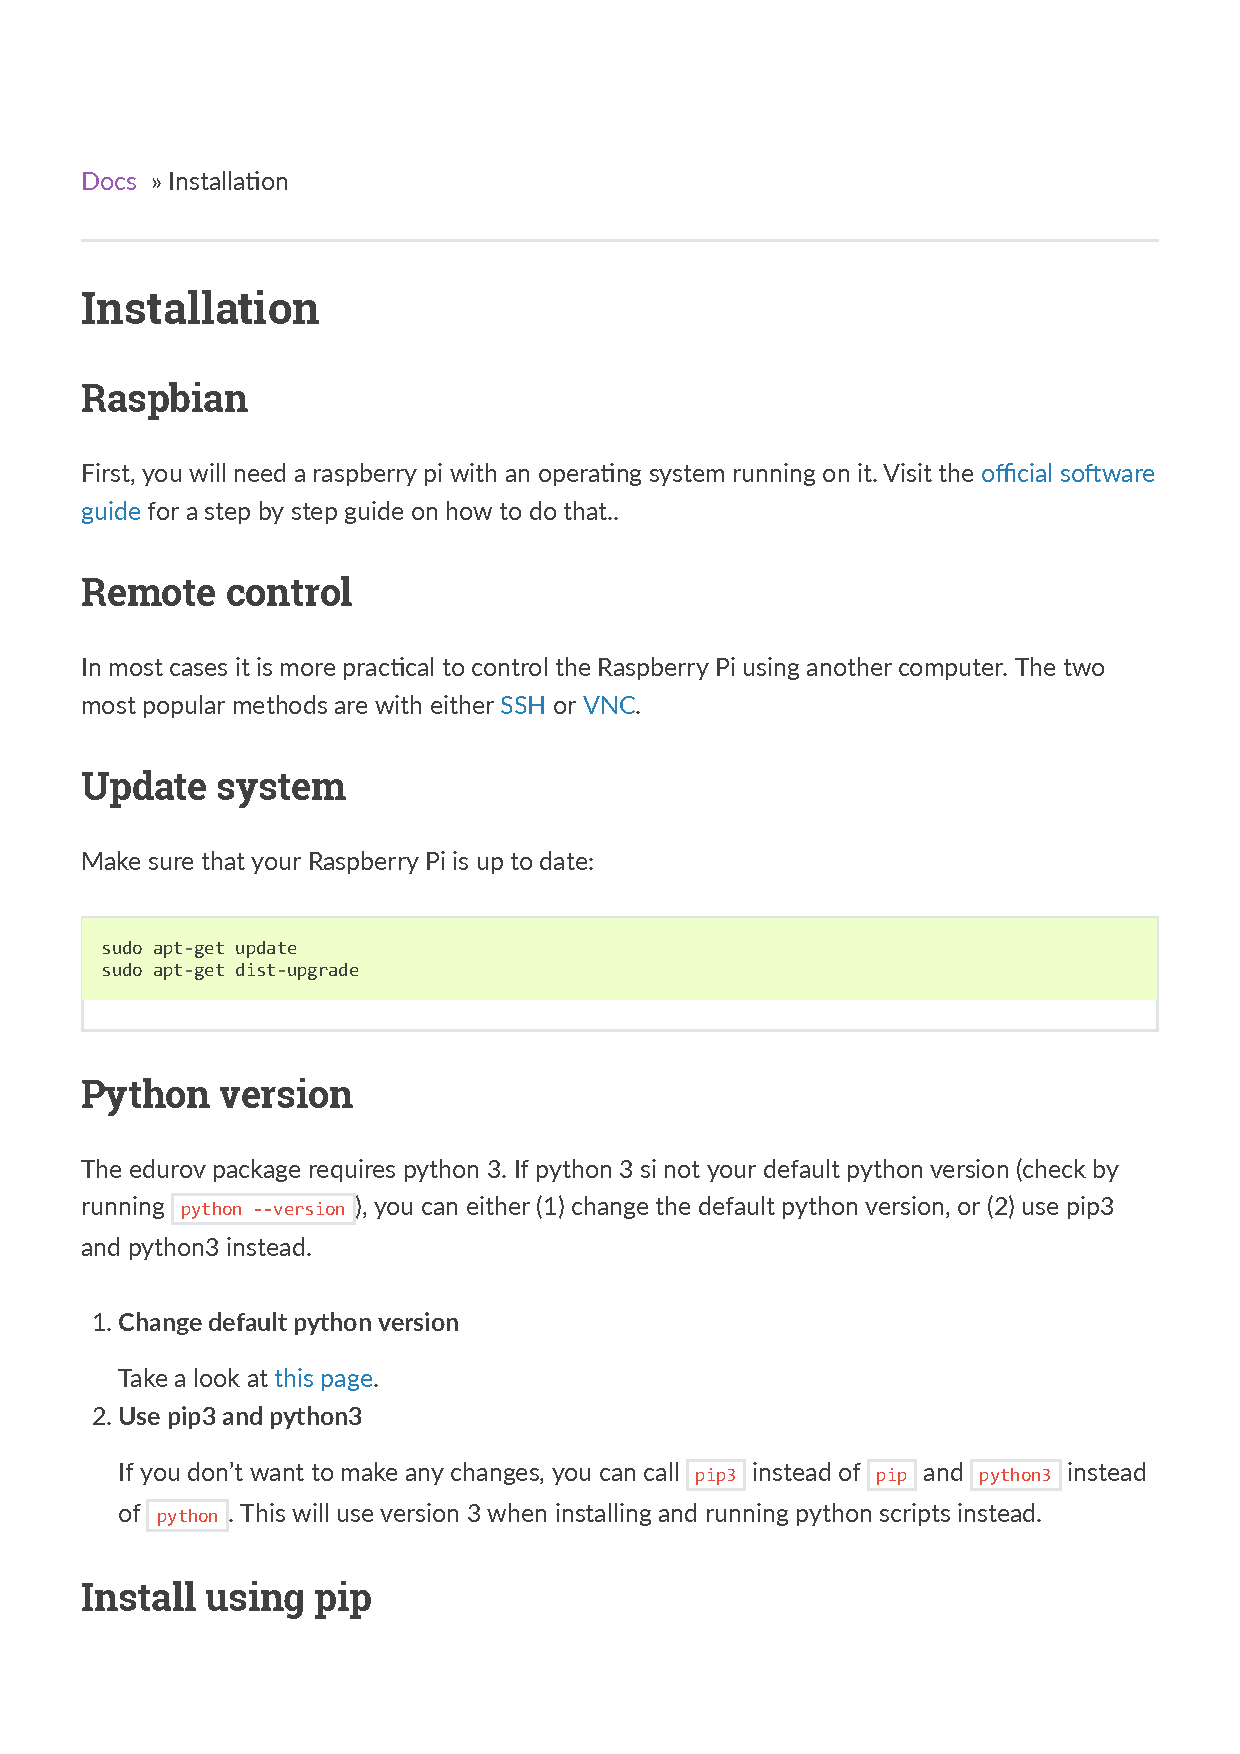
\includepdf[pages=-, frame=false, pagecommand={}, width=0.9\paperwidth]{./appendicies/docP2.pdf}
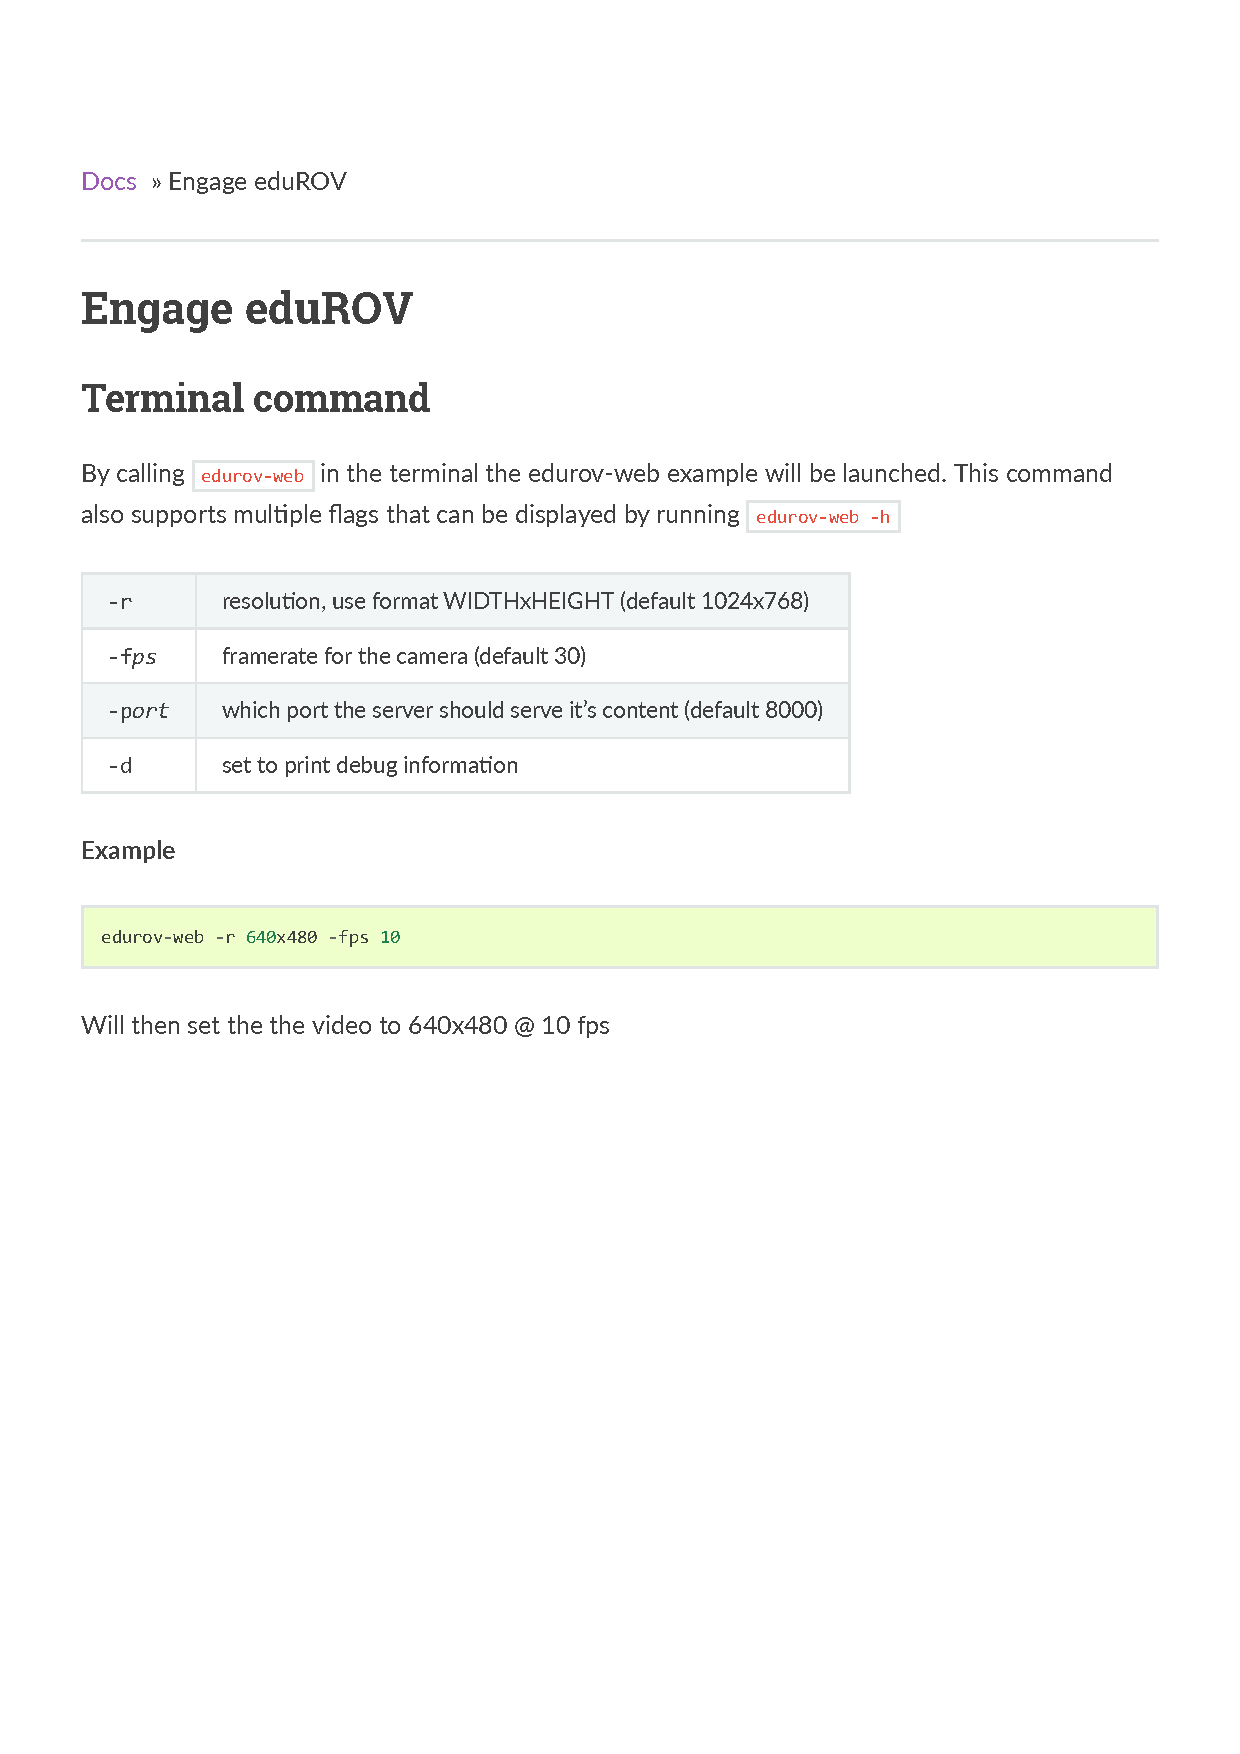
\includepdf[pages=-, frame=false, pagecommand={}, width=0.9\paperwidth]{./appendicies/docP3.pdf}
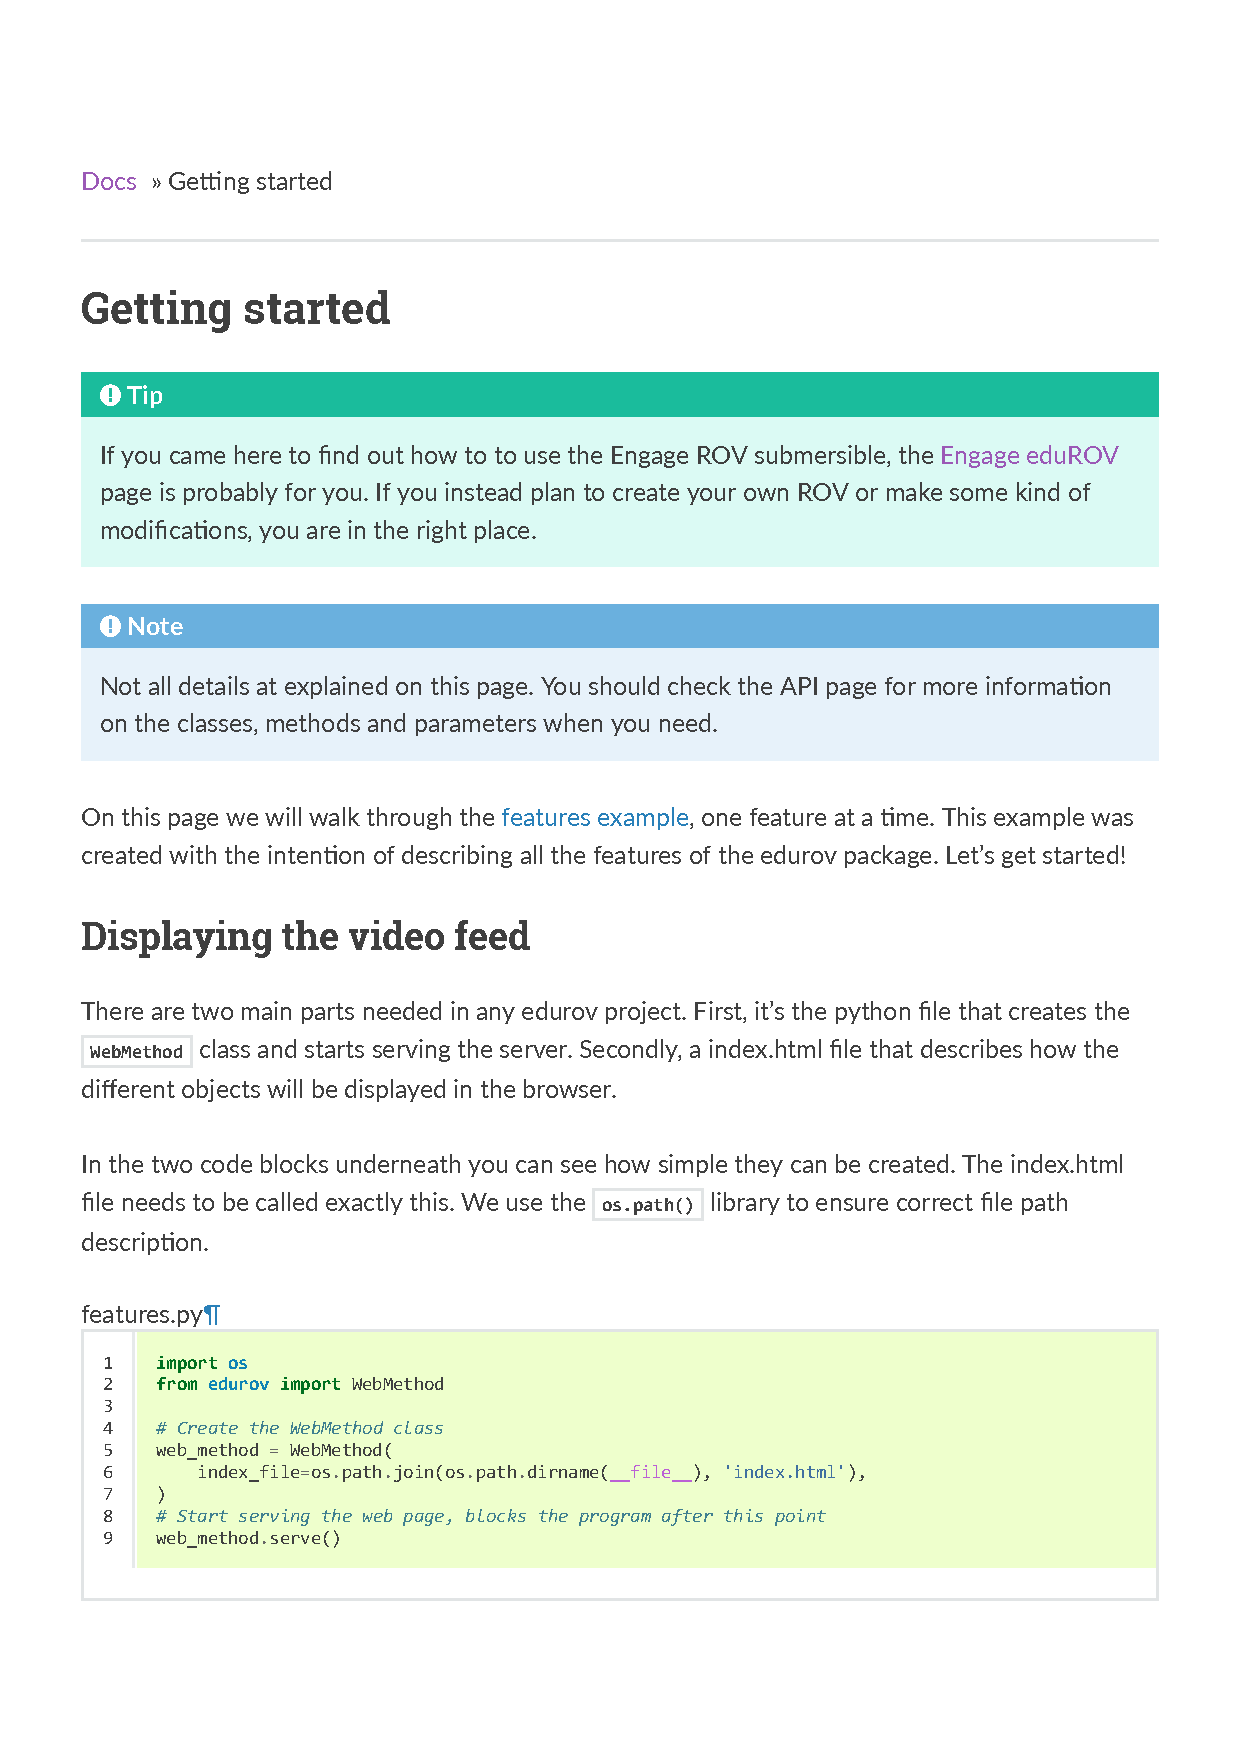
\includepdf[pages=-, frame=false, pagecommand={}, width=0.9\paperwidth]{./appendicies/docP4.pdf}
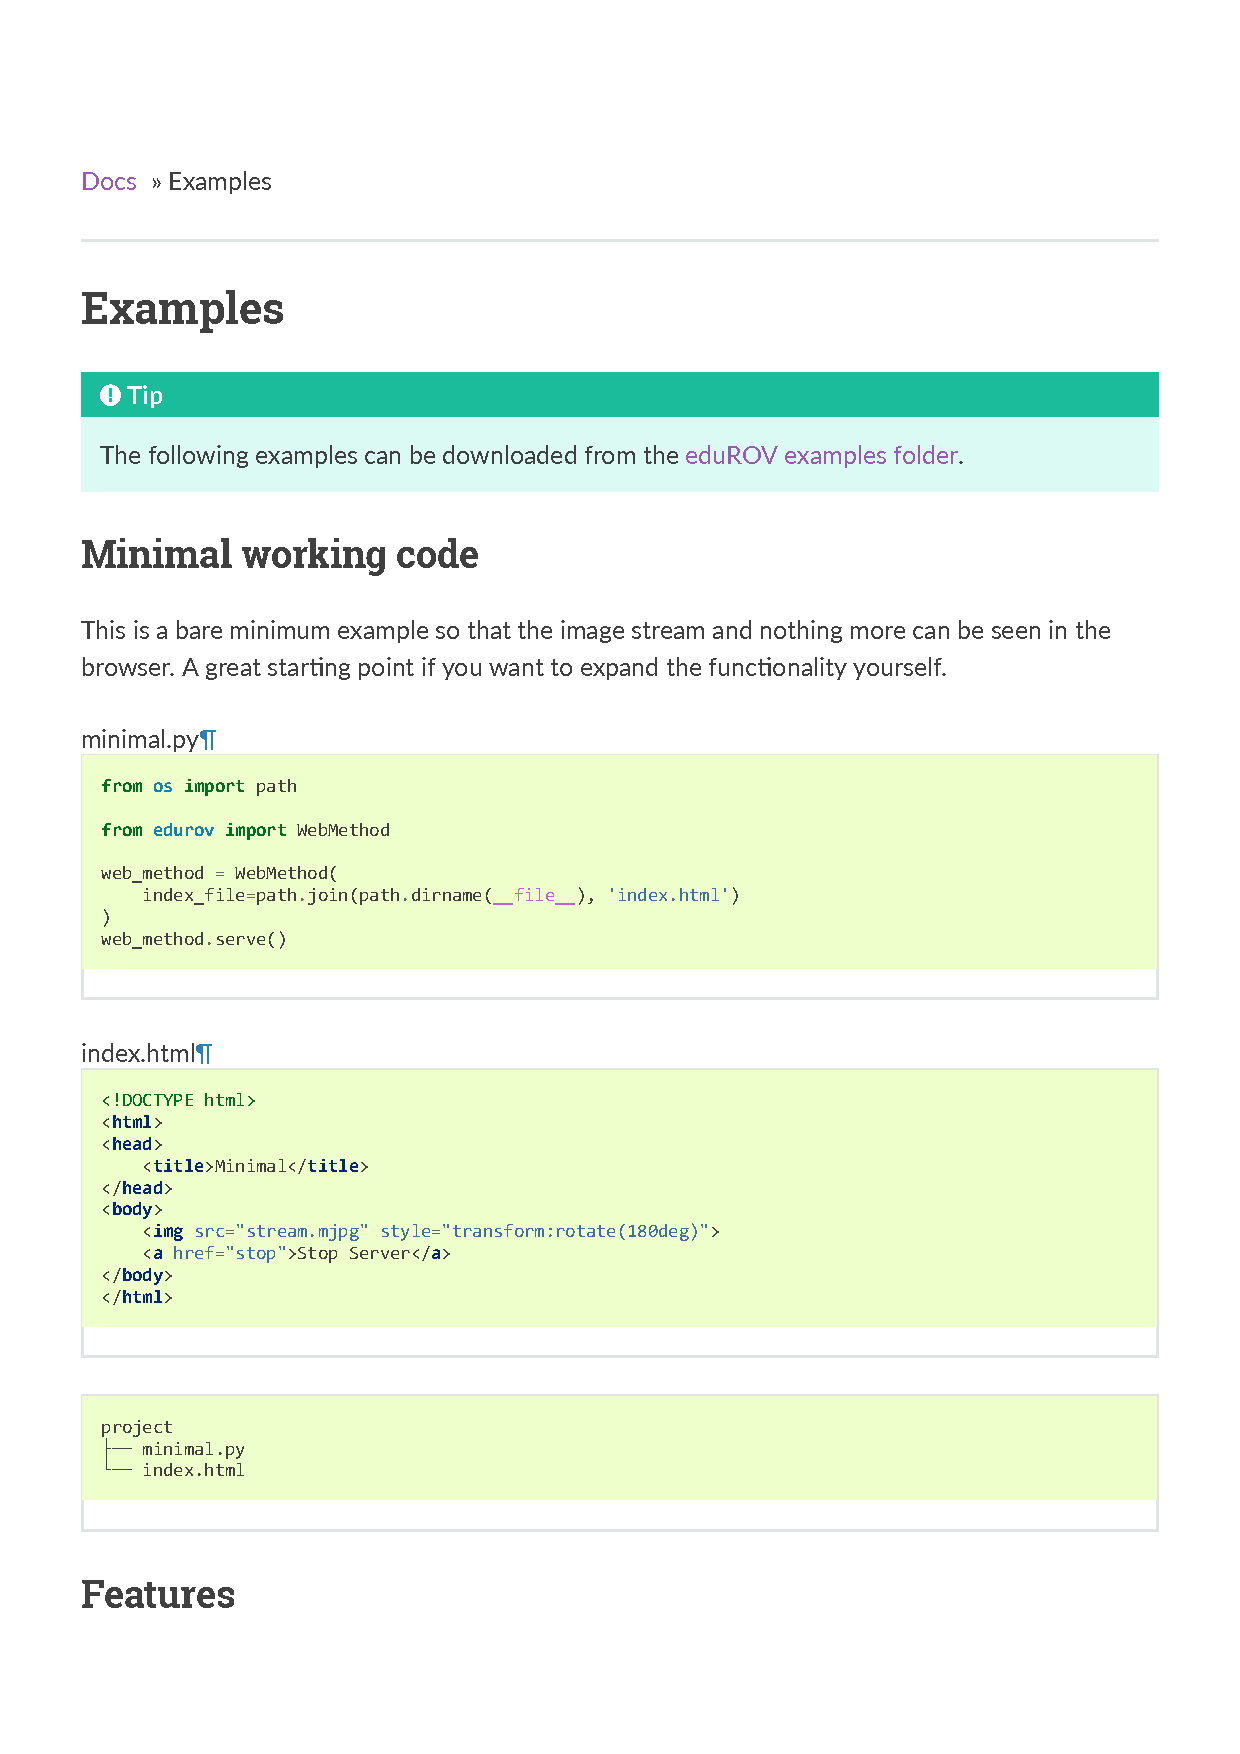
\includepdf[pages=-, frame=false, pagecommand={}, width=0.9\paperwidth]{./appendicies/docP5.pdf}
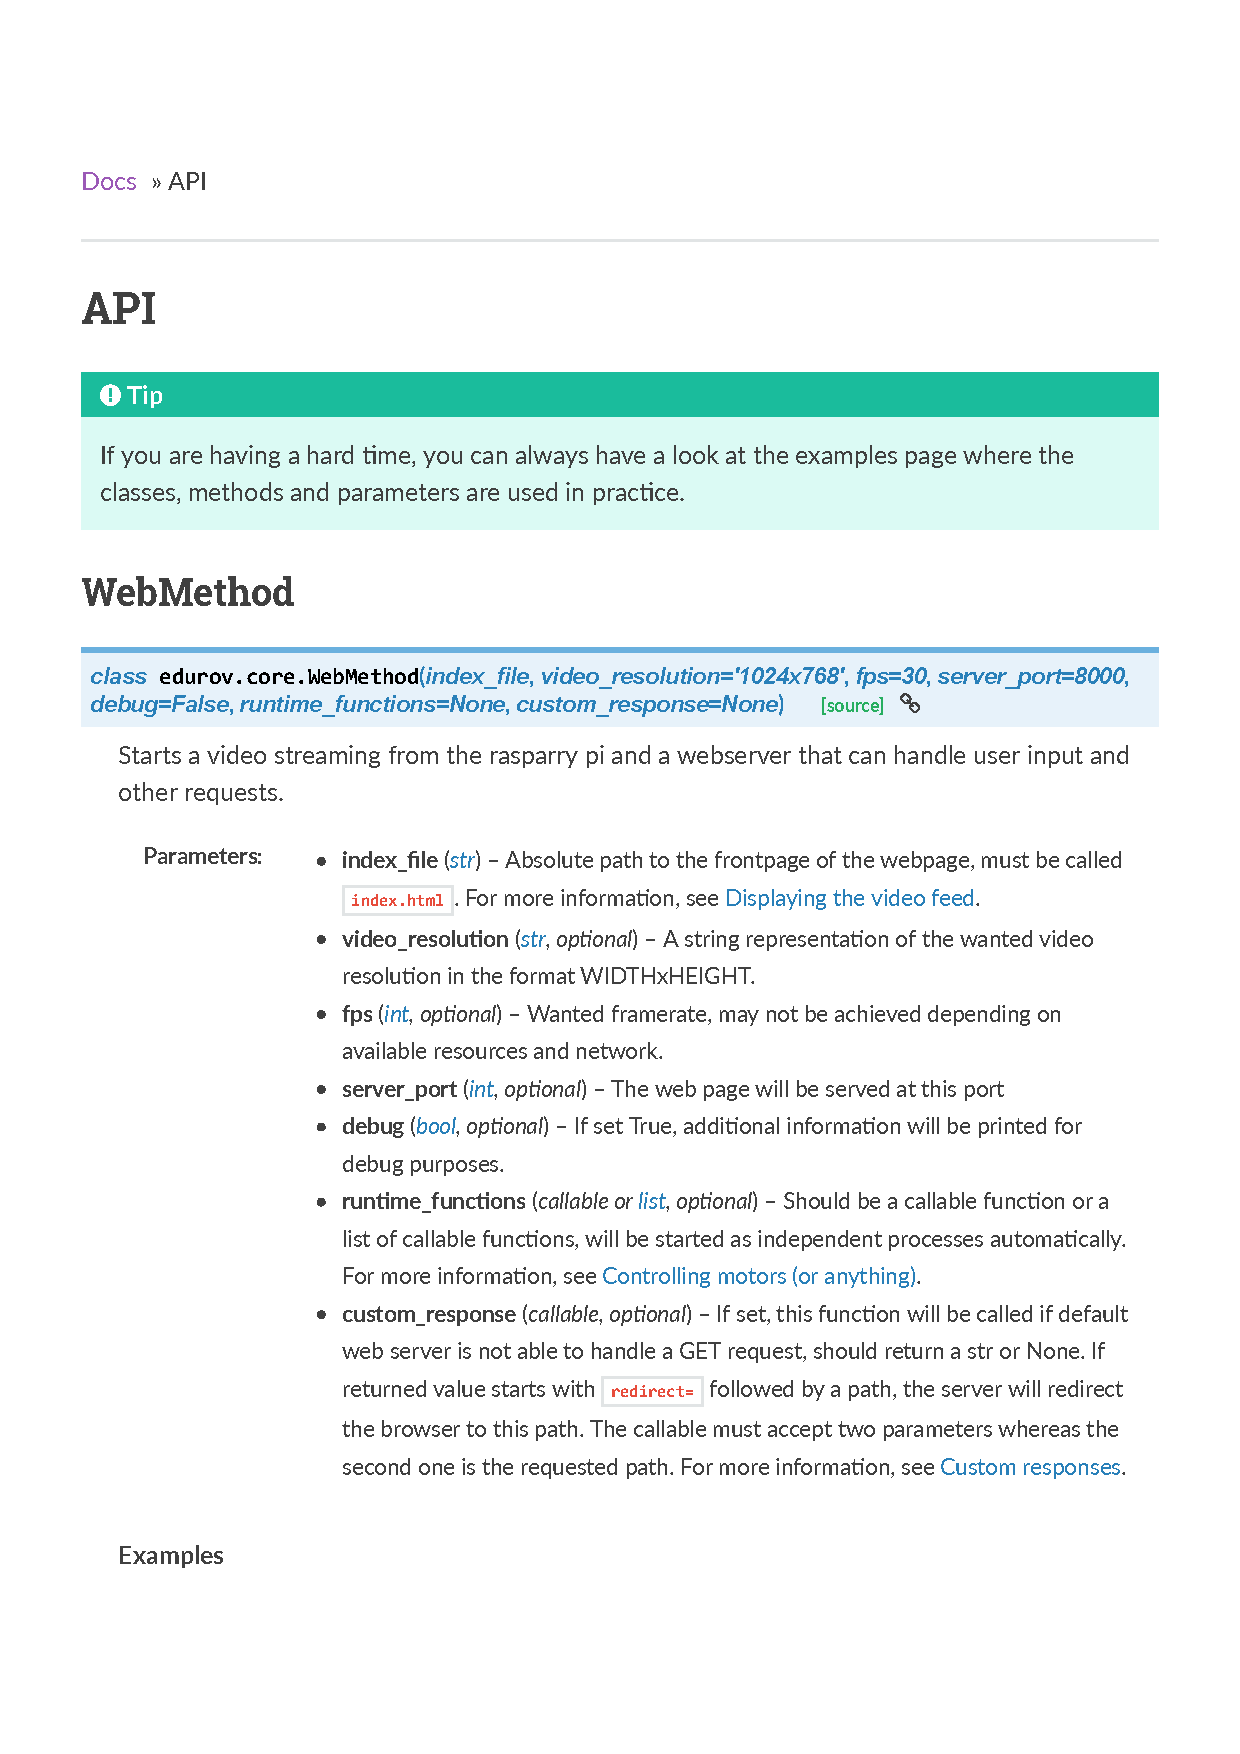
\includepdf[pages=-, frame=false, pagecommand={}, width=0.9\paperwidth]{./appendicies/docP6.pdf}

\chapter*{eduROV Package Code}\label{appCode}
\addcontentsline{toc}{section}{B eduROV Package Code}
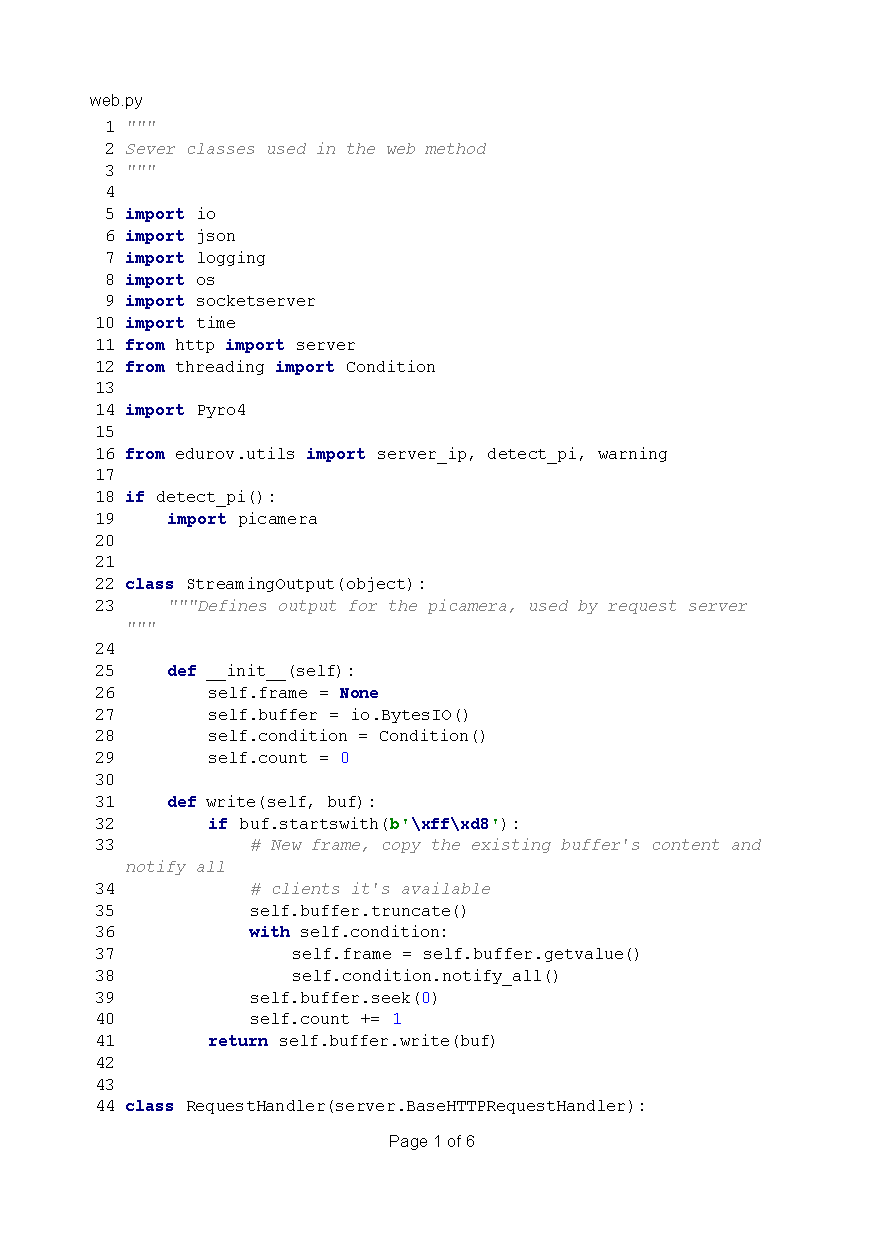
\includepdf[pages=-, frame=false, pagecommand={}, width=\paperwidth]{./appendicies/edurovCode.pdf}

\chapter*{Predictive Display Code}\label{appPredict}
\addcontentsline{toc}{section}{C Predictive Display Code}
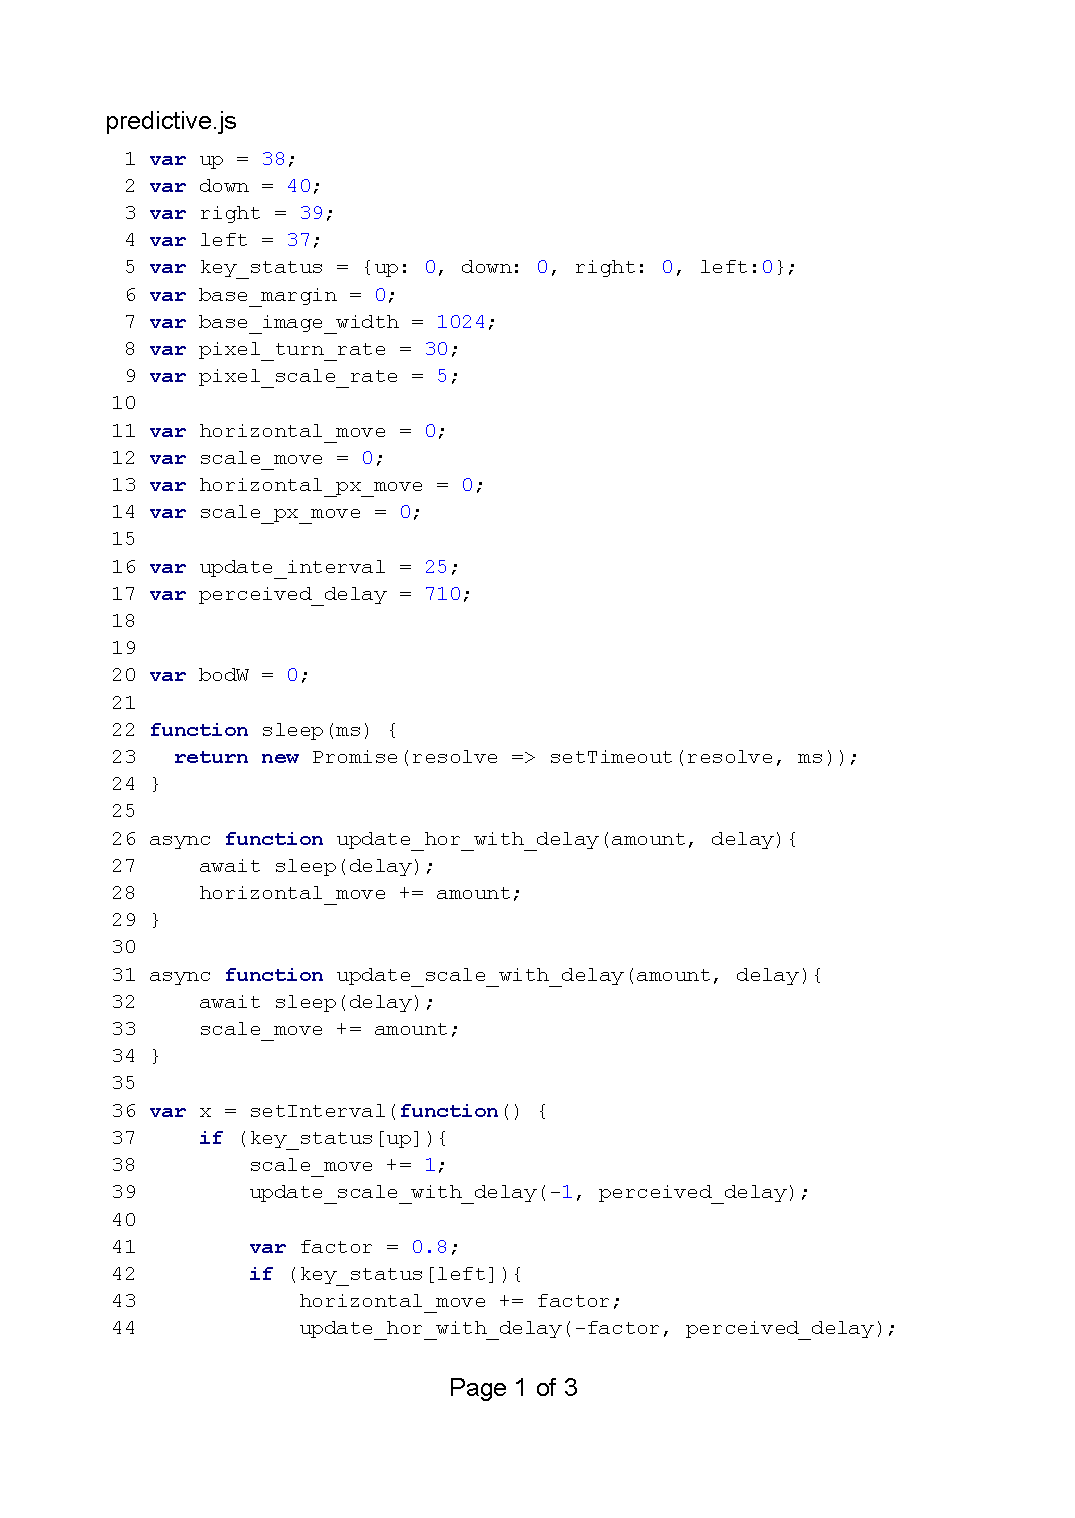
\includepdf[pages=-, frame=false, pagecommand={}, width=\paperwidth, offset=0cm -5mm]{./appendicies/predictor.pdf}

\chapter*{Experiment Info Page}\label{appInfo}
\addcontentsline{toc}{section}{D Experiment Info Page}
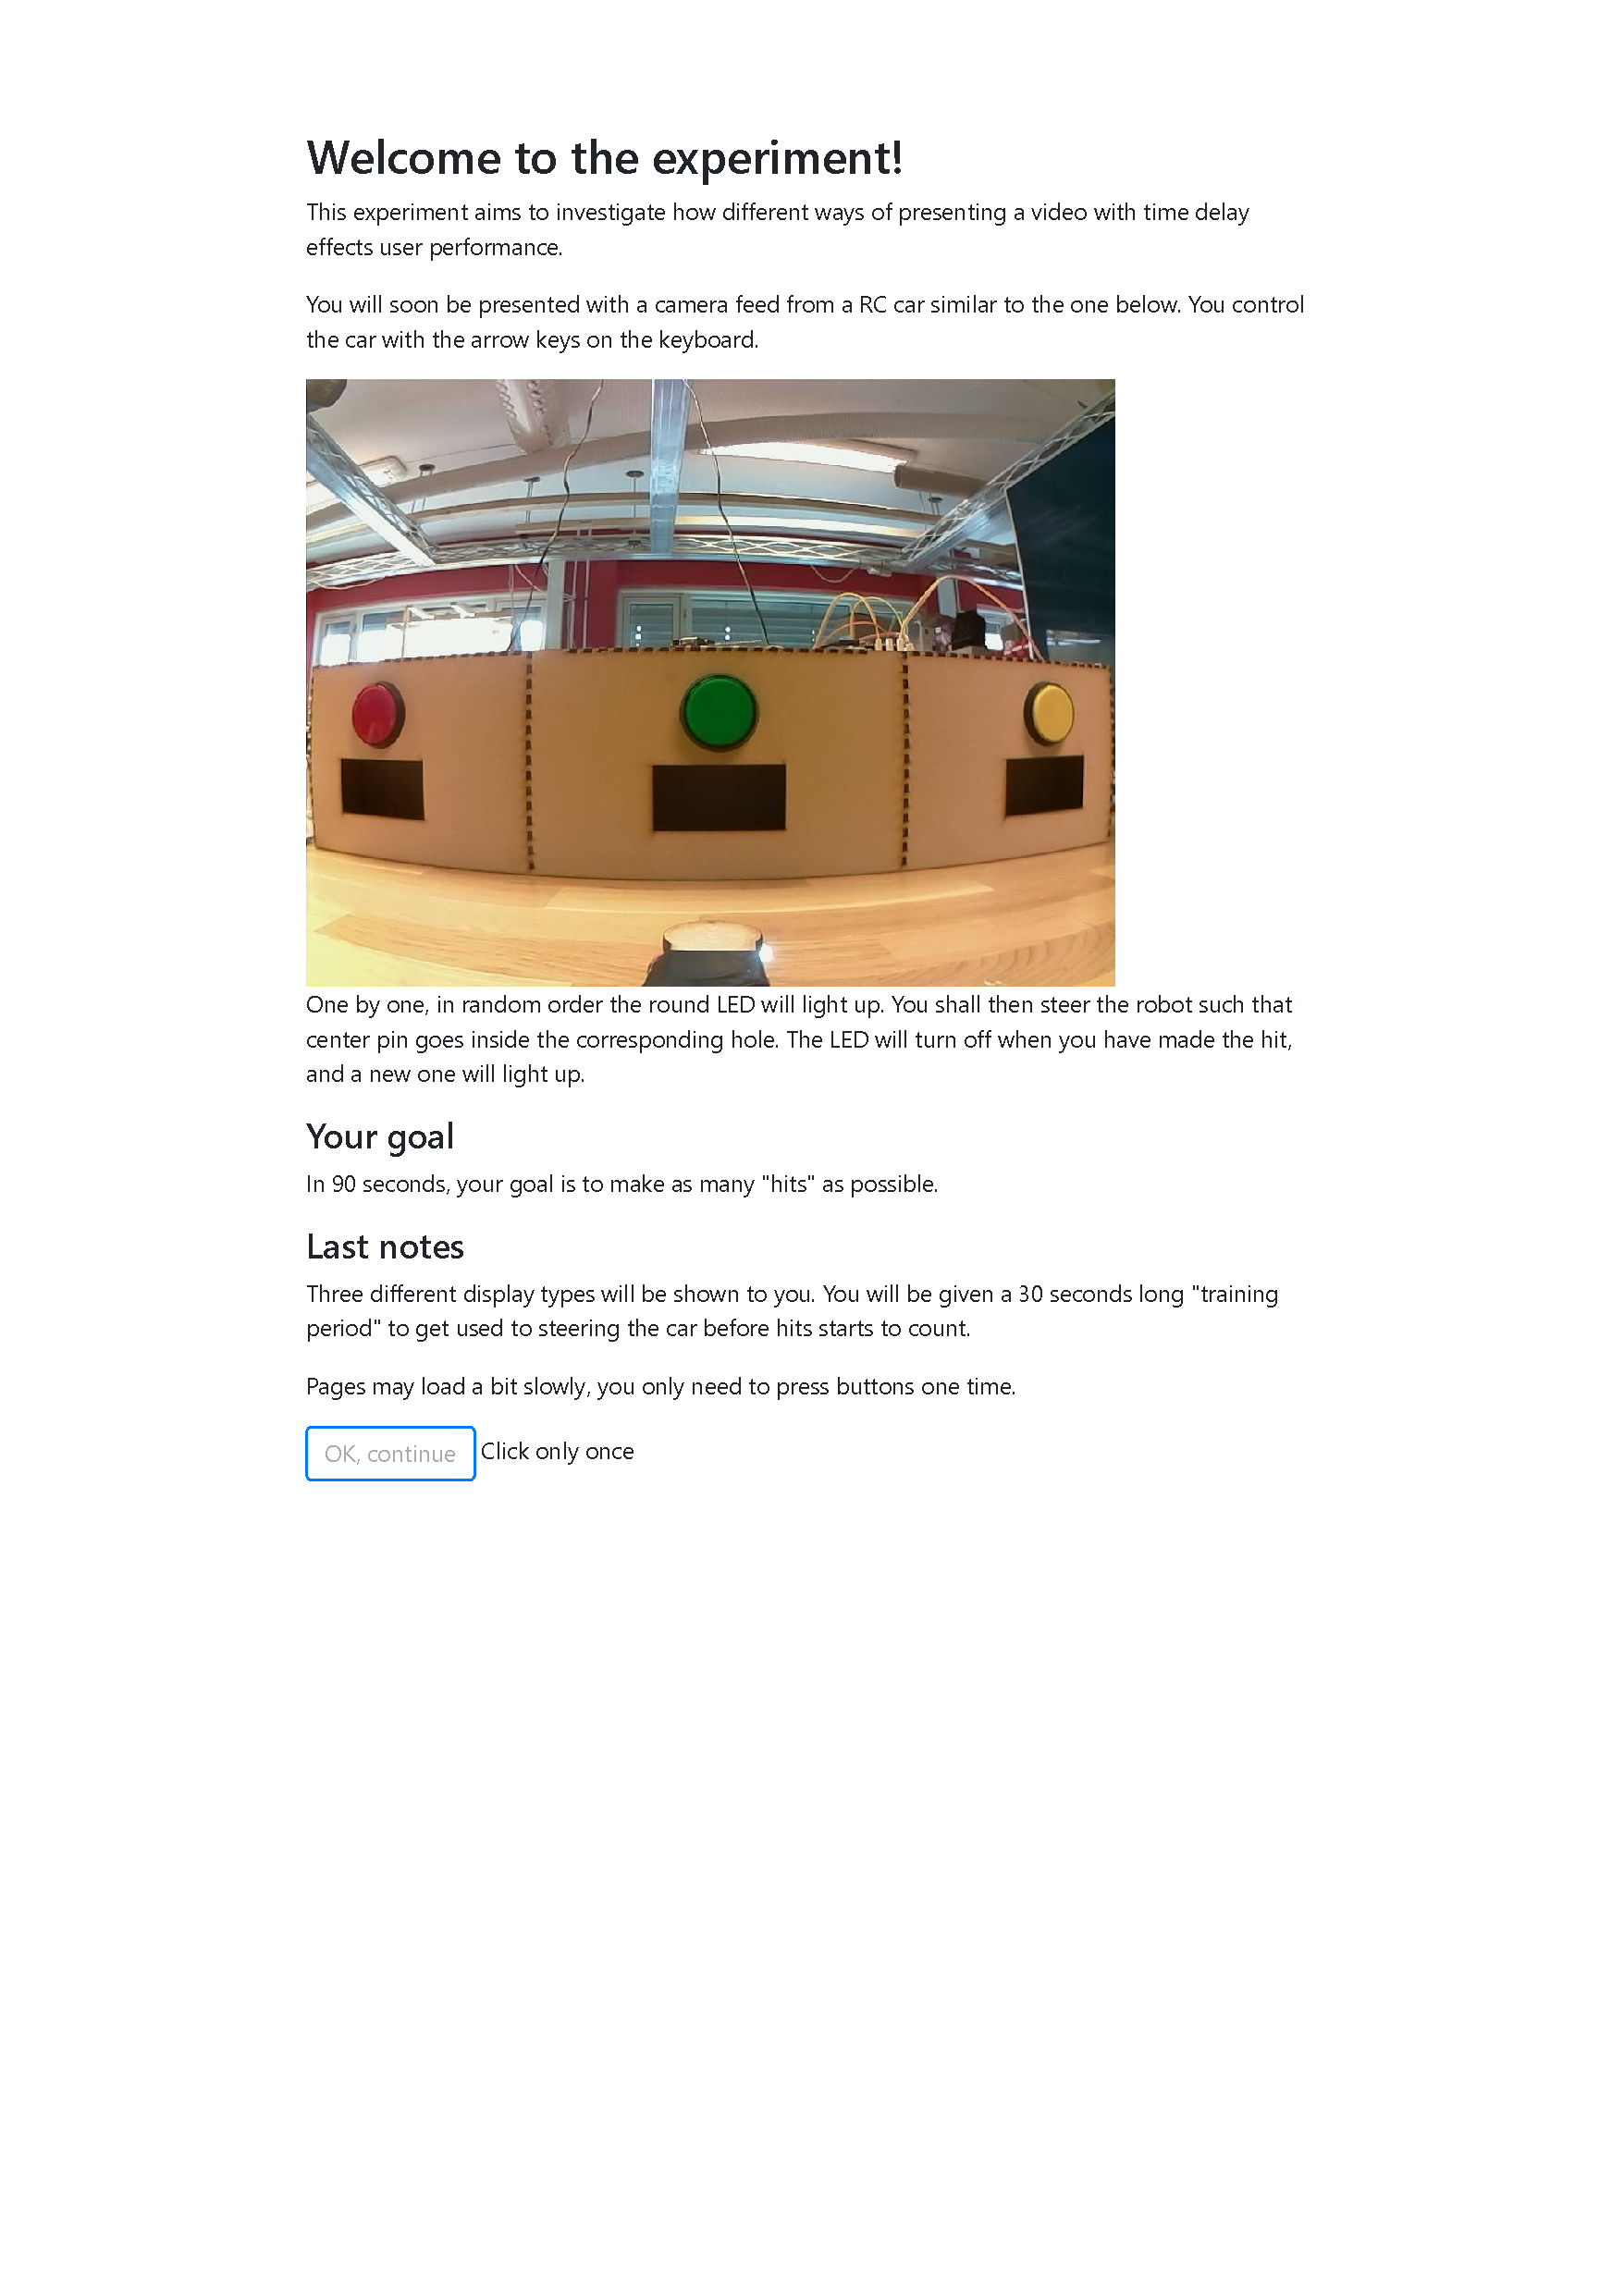
\includepdf[pages=-, frame=false, pagecommand={}, width=\paperwidth, offset=0cm -8mm]{./appendicies/infopage.pdf}

\chapter*{Experiment Questionnaire}\label{appSurvey}
\addcontentsline{toc}{section}{E Experiment Questionnaire}
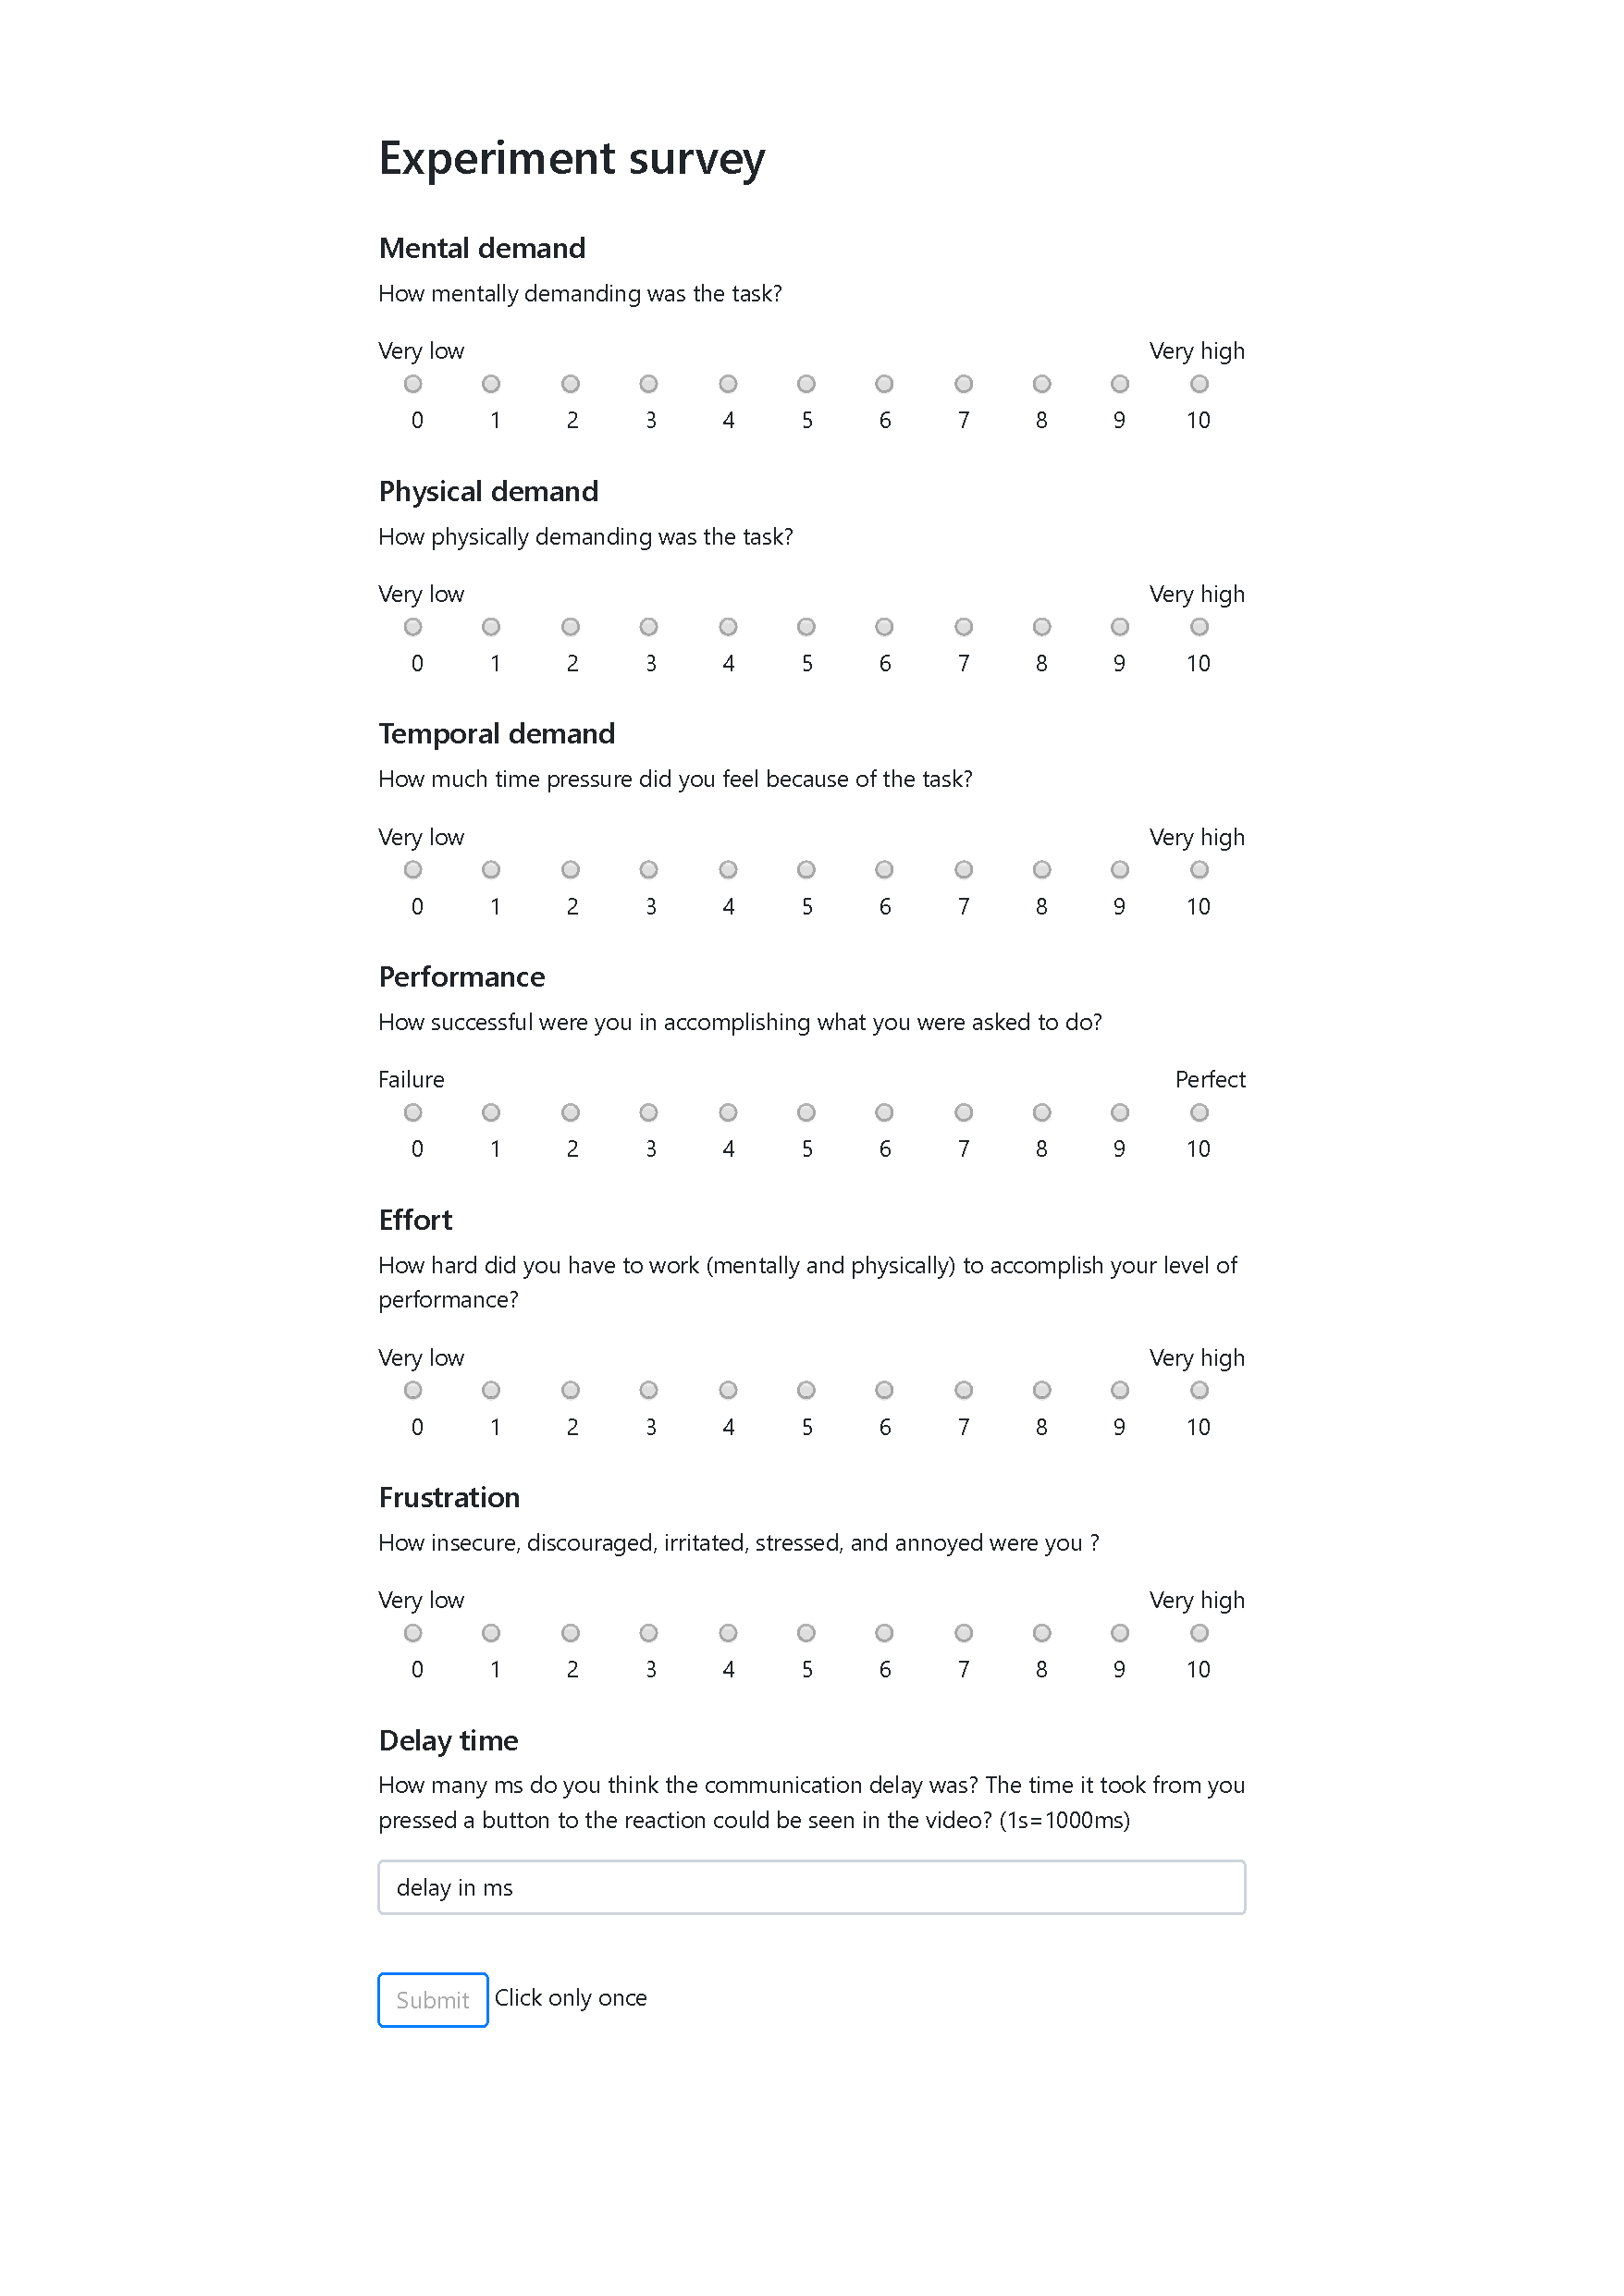
\includepdf[pages=-, frame=false, pagecommand={}, width=\paperwidth, offset=0cm -8mm]{./appendicies/survey.pdf}

\chapter*{Data Analysis Code}\label{appAnalysis}
\addcontentsline{toc}{section}{F Data Analysis Code}
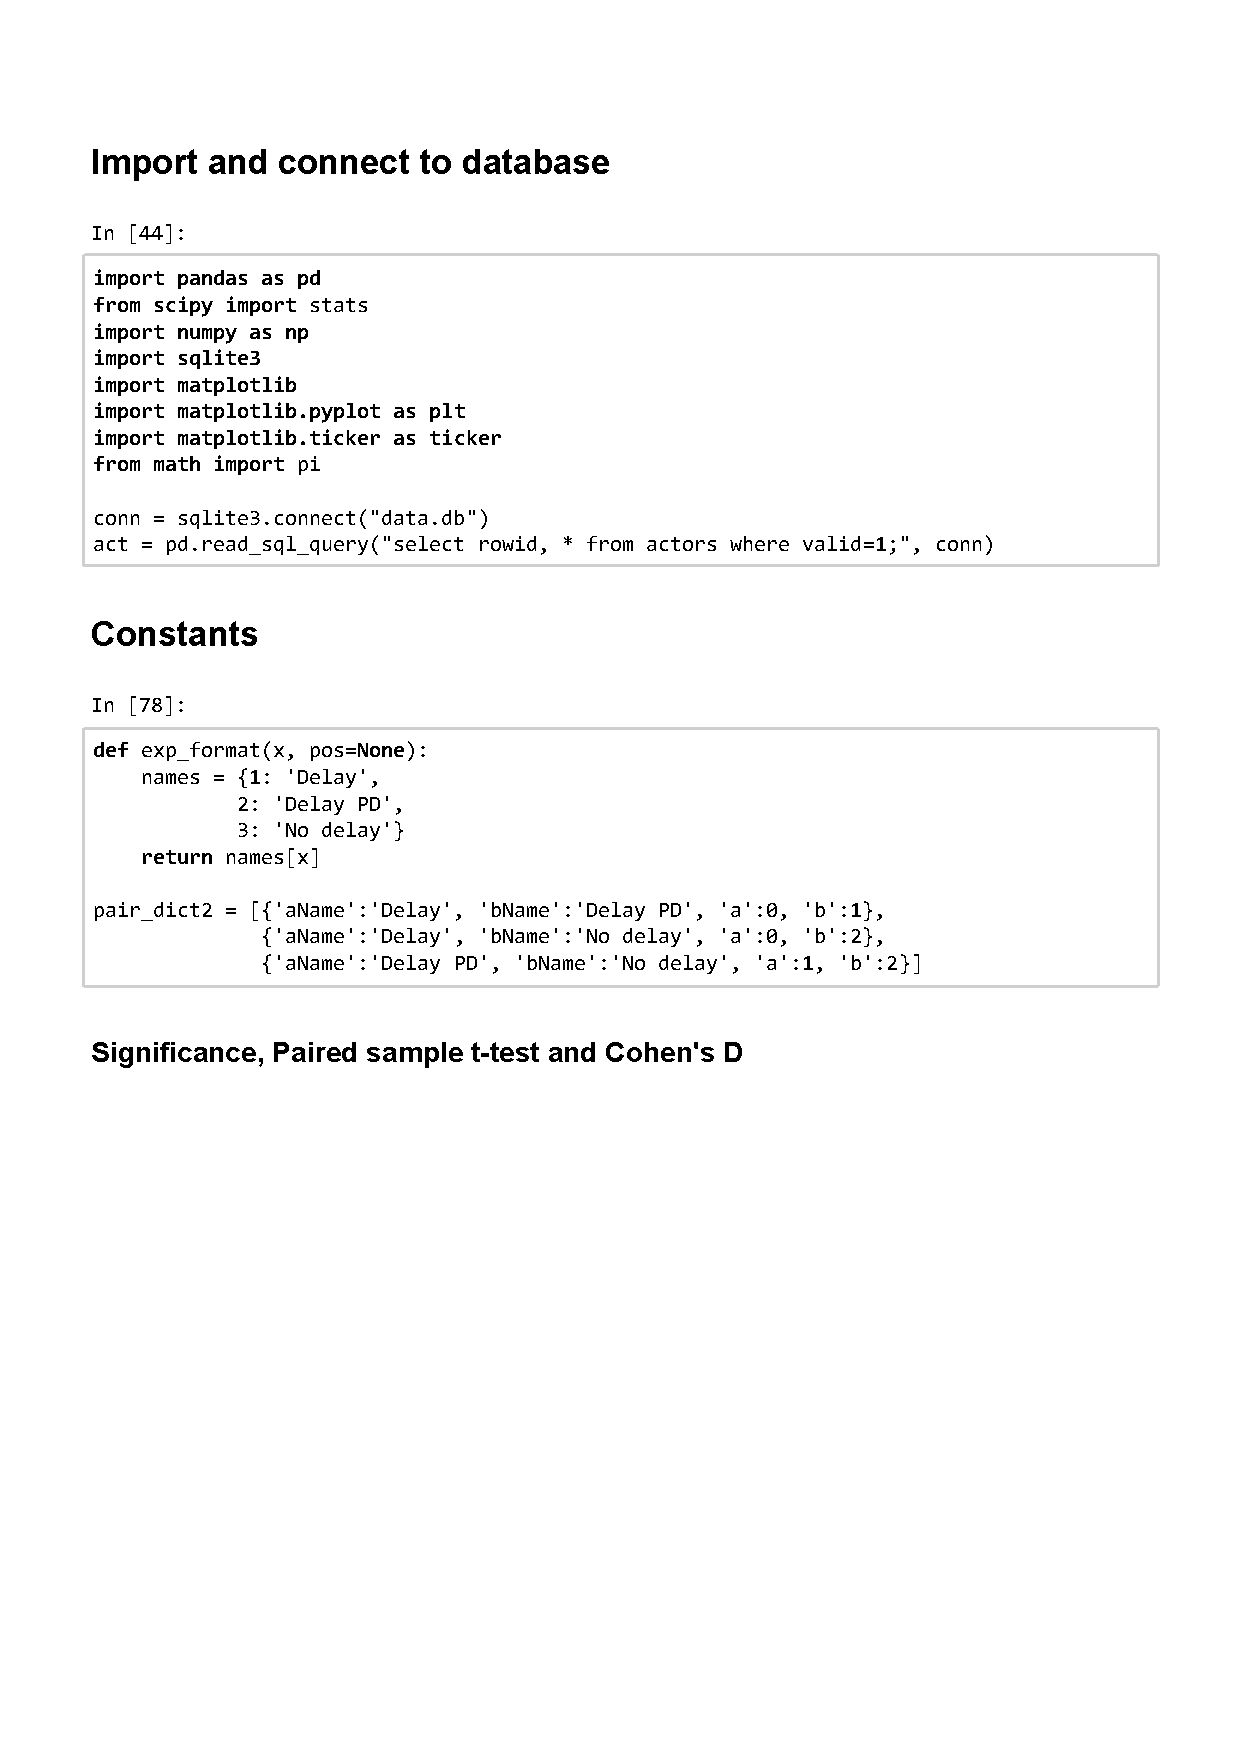
\includepdf[pages=-, frame=false, pagecommand={}, width=\paperwidth, offset=0cm -7mm]{./appendicies/analysis.pdf}

\chapter*{Collected Experiment Data}\label{appDatabase}
\addcontentsline{toc}{section}{G Collected Experiment Data}
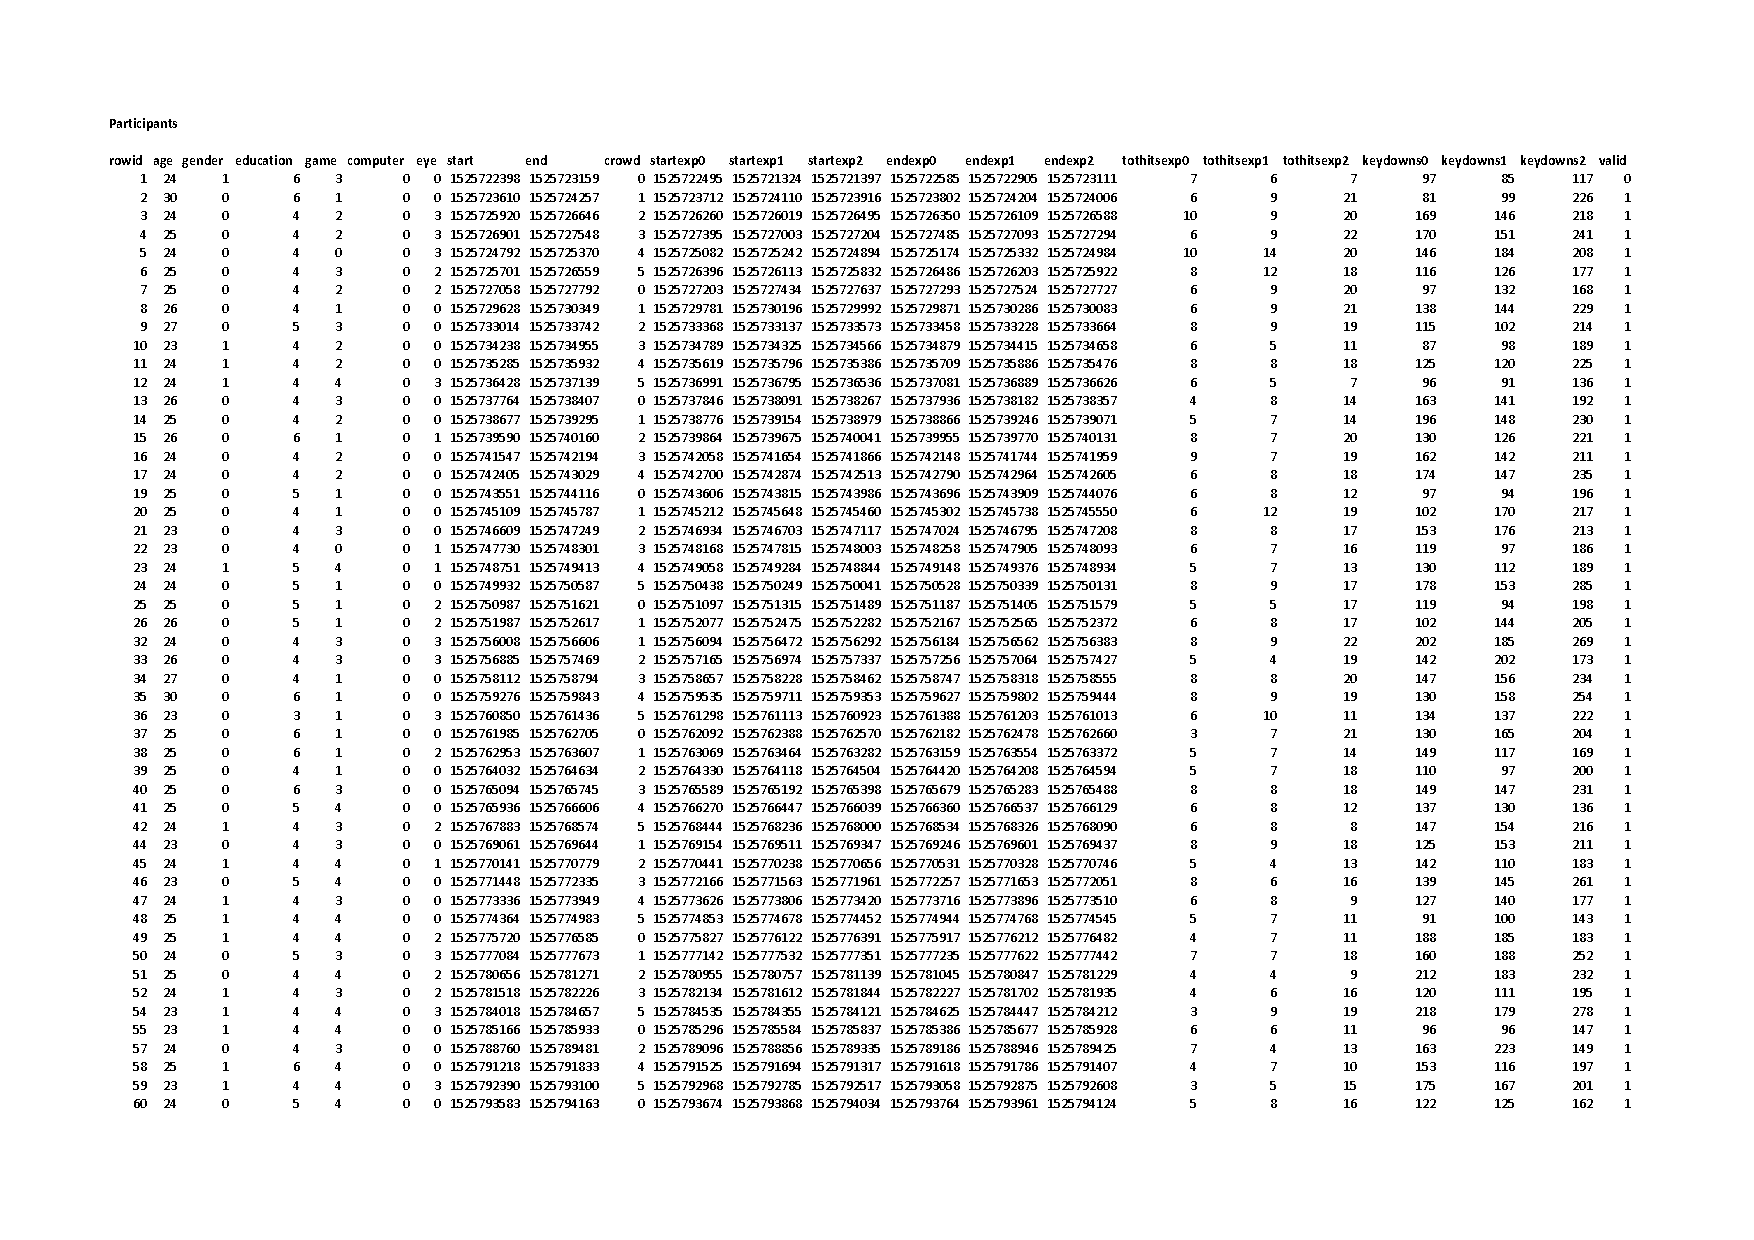
\includepdf[pages=-, frame=false, pagecommand={}, angle=90, width=\paperwidth, offset=0cm -7mm]{./appendicies/actors.pdf}
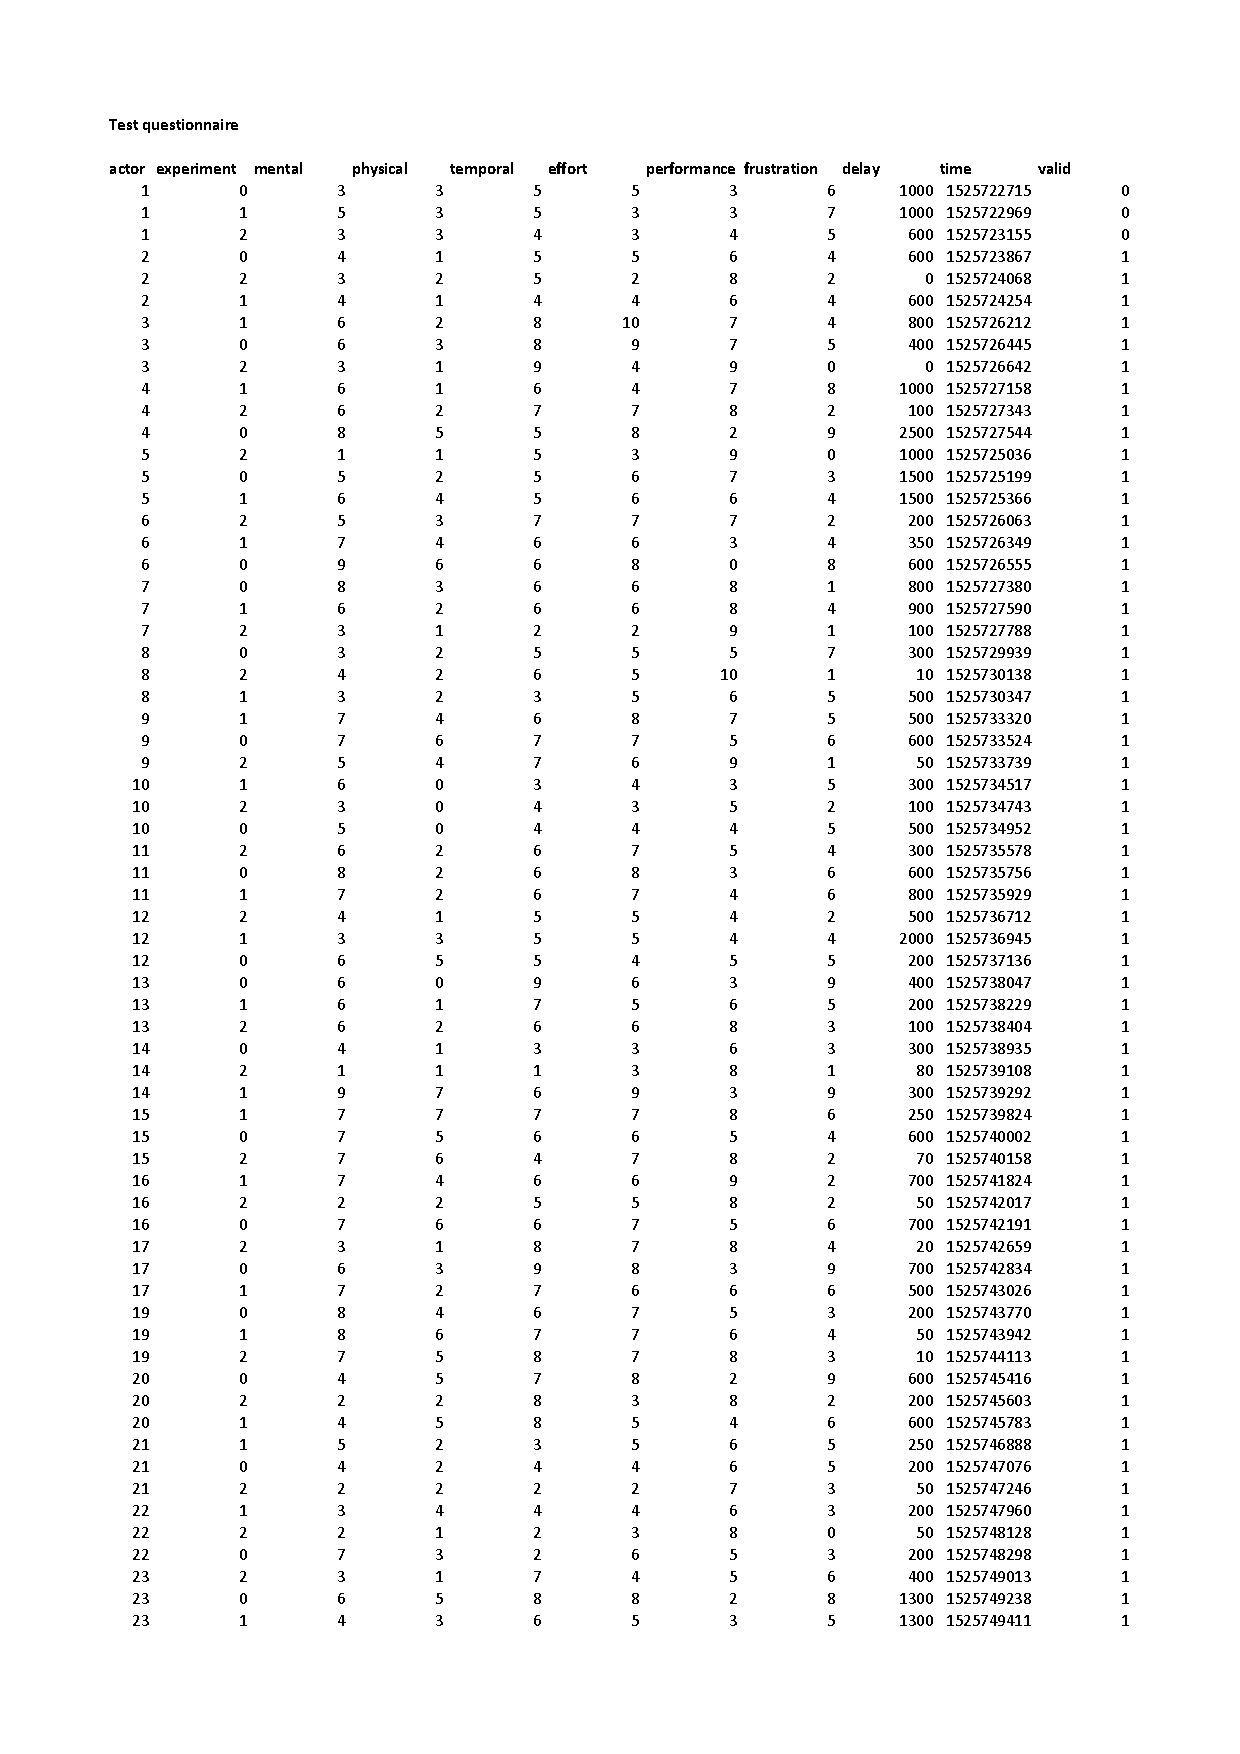
\includepdf[pages=-, frame=false, pagecommand={}, width=\paperwidth, offset=0cm -7mm]{./appendicies/surveyData.pdf}

\end{appendices}

\end{document}
